% !TeX TXS-program:compile = txs:///pdflatex/[--shell-escape]
% Le truc au-dessus pour avoir l'option shell-escape qui permet de faire du minted.
\documentclass[12pt]{article}

% Affichage ou non des reponses aux questions & exercices
\newif\ifDispRep
%\DispReptrue  % Show the text
\DispRepfalse % Hide the text

% Version du document
\newcommand{\versiondoc}{v0.3}

% Incorporation tous éléments de préambule communs à tous mes cours
% Sans chemin relatif parce que TexStudio lancé depuis un script qui prend en compte la variable d'environnement TEXINPUTS
\usepackage{CoursLFC}

% Eléments de l'en-tête et de la page de garde spécifiques à ce doc
\newcommand{\classe}{1\textsuperscript{ère} NSI}
\newcommand{\themecours}{Thème 6: Algorithmique}
\newcommand{\datedoc}{février 2024}

% Page de garde mise en page
\title
	{\vspace{3cm}
		{\Large
		\textit
			{
				\classe\hspace{0.1cm}
				\textemdash\
				\hspace{0.1cm}
				\themecours
			}
			
		\vspace{1cm}
		\huge{Algorithmique \& Mise au Point de Programmes} }
		 
		\vspace{1cm}
	}
\author{\etablissement}
\date{
	\auteur,
	\datedoc,
	\footnotesize{\textit{\versiondoc}} 
	\vspace{2cm}
	}

% Header & Footer
\lfoot{\etabshort}
\cfoot{\thepage}
\rfoot{\classe, \anneescol}
\renewcommand{\footrulewidth}{0.2pt}
\lhead{}
\chead{}
\rhead{}
\renewcommand{\headrulewidth}{0pt}

\begin{document}
	
	\maketitle
	% pas de footer sur la première page
	\thispagestyle{empty}
		
	\section*{}
		{\noindent
		\resumecours
		}
	
	\vspace{2cm}
	\begin{MaReponse}
		\centering
		\vspace{\baselineskip}
		\textbf{Document de cours incluant les réponses aux exercices.}
		\vspace{\baselineskip}
	\end{MaReponse}
		
	\pagebreak	
	\tableofcontents
	
	\pagebreak
	
	% Début du contenu du document

	\section{Point d'étape -- où est-on / où va-t-on?}
	\subsection{Ce qu'on a couvert jusqu'à présent}
	
	\begin{itemize}
		\item Rudiments de l'architecture physique d'un ordinateur -- le modèle de Von Neumann.
		\item Mise en jambes sur de l'écriture de code: réalisation d'une page Web en HTML.
		\item Introduction à Python, et plus spécifiquement:
		\begin{itemize}
			\item Ce qu'on appelle ses "constructions élémentaires" -- variables, fonctions, conditions \& embranchements, boucles...
			\item Les types et valeurs de base: entiers (naturels et relatifs), flottants (réels), chaînes de caractères et booléens (qu'on n'a que brièvement abordés pour l'instant).
			\item Un type dit "construit" -- les listes.
		\end{itemize}
		\item Un peu de théorie: la représentation des types et valeurs de base en machine (les entiers naturels et relatifs, les réels, les alphanumériques).
		\item Un peu plus de théorie: introduction à la logique booléenne (que l'on n'a couverte que très rapidement -- on y reviendra en fin d'année).
		\item Un retour à la pratique: le traitement de données en table, la manipulation de fichiers dans Python, et des types de données plus complexes --- les dictionnaires, les listes de dictionnaires...
	\end{itemize}
	
	\subsection{Ce dont on va parler dans ce nouveau chapitre}
	On a donc fait des "sauts" de la théorie vers la pratique, puis vers la théorie de nouveau --- pour finalement atterrir ici, dans ce chapitre sur l'algorithmique qui se trouve presque exactement au "milieu" de cet axe théorie--pratique.
	
	Comme je vous l'ai dit à plusieurs reprises dans les parties précédentes -- et spécialement dans celle portant sur le traitement de données en table, l'algorithmique, vous en faites déjà: je vous pose des problèmes par le biais de notebooks Jupyter dans Capytale v2 et vous réfléchissez à comment les résoudre. Dit autrement, \textit{vous concevez des algorithmes}.
	
	Ce que l'on va faire dans ce nouveau chapitre c'est formaliser cette démarche, la structurer, puis étudier quelques exemples d'algorithmes beaucoup plus avancés que ce que l'on a vu jusqu'à présent.
	
	Spécifiquement, on va parcourir le chemin suivant:
	\begin{itemize}
		\item Introduction à l'algorithmique -- étapes de conception et de rédaction d'un algorithme;
		\item Pratique: tests d'algorithmes / de programmes;
		\item Preuve d'algorithmes;
		\item Complexité d'algorithmes;
		\item Etude de certains algorithmes spécifiques:
		\begin{itemize}
			\item Algorithmes de tri - par sélection, par insertion;
			\item Algorithme de recherche dichotomique dans un tableau;
			\item Algorithmes gloutons;
			\item Algorithmes des k plus proches voisins -- algorithme d'apprentissage, "machine learning".
		\end{itemize}
		\item Pratique: mise au point de programmes; programmation défensive.
	\end{itemize}
	
	\subsection{Comment on va procéder}
	Comme dit plus haut, on est ici à la frontière entre la théorie et la pratique -- on va donc avoir un fonctionnement hybride en classe:
	 \begin{itemize}
	 	\item \textbf{Prise de notes essentielle} --- vous commencez à connaître les cours que je vous fournis, il sont \textit{très} longs. Ils doivent vous servir de référence, vous permettre surtout de bien revoir les corrections d'exercices, mais votre savoir, lui, doit venir de votre prise de notes;
	 	\item Plusieurs exercices sur papier qu'on fera en classe et dont il sera très important que vous gardiez une trace;
	 	\item En parallèle et en complément, quelques applications / exercices sur machine.
	 \end{itemize}
	
	\subsection{Comment réviser / préparer les contrôles?}
	
	Comme pour les autre chapitres de cours de NSI, les deux choses les plus importantes que vous devez acquérir pour être en mesure de bien réussir les contrôles sont:
	\begin{itemize}
		\item Connaître et comprendre les notions présentées dans le cours (et en particulier les définitions);
		\item Être capable de faire tous les exercices présents dans ce cours et également dans le cahier d'exercices qui l'accompagne.
	\end{itemize}
	 
	 Plus spécifiquement, chaque section de ce cours se termine par un encart (sur fond vert) intitulé "À Savoir \faExchange \ À Réviser" dans lequel je vous explique plus en détails ce qu'il y a à retenir de la section en question.
	 
	 En tout état de cause mon conseil principal pour les révisions est de prendre la version de ce cours et du cahier d'exercices qui ne contient \textit{\textbf{pas}} les solutions, vous exercer à faire les exercices qui sont dedans, puis vérifier les réponses dans la version qui contient les solutions.
	 
	 Bon courage!
	 
	 \pagebreak
	 
	 \section{Introduction à la conception d'algorithmes}
	 
	 Quelques questions pour commencer...
	 
	 \MaQuest{Qu'est-ce qu'un algorithme (indice: c'est constitué de trois parties)? }
	 \begin{MaReponse}
	 	Un algorithme est une \textbf{suite finie d'instructions} permettant de \textbf{résoudre un problème}. Il est structuré en trois parties:
		 \begin{alphenum}
		 	\item L'entrée des données;
		 	\item Le traitement des données;
		 	\item La sortie des données 
		 \end{alphenum}
	\end{MaReponse}
	
	\MaQuest{Parmi les éléments suivants, qu'est-ce qui est un algorithme, qu'est-ce qui n'en est pas?
		\begin{alphenum}
			\item Une recette de gâteau au chocolat;
			\item La liste des présidents de la V\textsuperscript{ème} République;
			\item Les règles du jeu d'échecs;
			\item Les règles à appliquer pour résoudre une équation du 2\textsuperscript{nd} degré;
			\item Les instructions de montage d'un meuble Ikea.
		\end{alphenum}
	}
	
	\begin{MaReponse}
		\begin{alphenum}
			\item Oui c'en est un -- ingrédients en entrée, étapes de confection, gâteau en sortie. C'est bien la résolution d'un problème (en l'occurrence "comment fabriquer un gâteau au chocolat?").
			\item Non ce n'en est pas un -- c'est une liste d'informations, pas des étapes à suivre.
			\item Ce n'en est pas un non plus -- ce n'est qu'une liste de principes. En revanche on pourrait les utiliser pour mettre en \oe{}uvre un algorithme qui joue aux échecs (et résoud le problème "comment jouer -- et gagner -- une partie d'échecs?).
			\item Oui c'en est un -- c'est même écrit dans la description ("résoudre").
			\item Oui c'en est un également.
		\end{alphenum}
	\end{MaReponse}
	
	Donc, pour reprendre:
	\begin{MaDef}{algorithme}
		Un algorithme est une \textbf{suite finie d'instructions} permettant de \textbf{résoudre un problème}. Il est structuré en trois parties:
		\begin{alphenum}
			\item L'entrée des données;
			\item Le traitement des données;
			\item La sortie des données 
		\end{alphenum}
	\end{MaDef}
	
	\begin{MaDef}{l'algorithmique}
		L'algorithmique est:
		\begin{itemize}
			\item La conception (et la production) d'algorithmes;
			\item Leur étude -- leur analyse, la mesure de leur fiabilité (est-ce qu'il répond vraiment au problème posé?) et de leur efficacité (est-ce qu'il le fait en un temps acceptable?).
		\end{itemize}
	\end{MaDef}
	
	Nous allons dans ce cours nous intéresser à ces deux composantes, en commençant, dans ce chapitre, par la première dont les étapes peuvent se résumer ainsi:
	\begin{enumerate}
		\item Énoncé d'un problème à résoudre;
		\item Spécification de l'algorithme -- nom, entrées, sorties;
		\item Explicitation de la démarche en pseudo-code -- description du traitement des données qui va permettre de résoudre le problème;
		\item Traduction en langage de programmation.
	\end{enumerate}
	
	La 1\textsuperscript{ère} et la 4\textsuperscript{ème} étape sont à la marge de notre propos ici:
	\begin{itemize}
		\item L'énoncé d'un problème à résoudre par le biais d'un programme informatique est une activité à part entière (souvent appelée "expression de besoin" dans le monde professionnel). Vous y avez un petit peu touché dans le cadre de vos projets, mais dans l'ensemble, dans le contexte de la NSI, les problèmes vous sont posés -- et votre rôle consiste à savoir les résoudre;
		\item La traduction en langage de programmation, que dans le contexte de la NSI nous réalisons en Python, a fait l'objet d'un pan du cours distinct; nous allons évidemment y revenir en partie ici, mais la syntaxe Python n'est pas l'objet de notre étude ici.
	\end{itemize}
	
	\subsection{Écrire un algorithme: spécification}
	
	Avant d'écrire un algorithme il faut bien définir ce que l'on veut faire et à partir de quoi; il s'agit de donner \textbf{une spécification au problème}. Pour cela on doit:
	\begin{itemize}
		\item Donner un nom explicite à l’algorithme --- \textit{par exemple \texttt{CuissonGateauChocolat}};
		\item Décrire les conditions d'utilisation de l'algorithme, les données qu'il attend en entrée et les conditions dans lesquelles il va pouvoir être exécuté, sa \textbf{\textit{précondition}} --- \textit{par exemple "\texttt{Beurre et Lait non périmés}"}:
		\item De même, décrire le résultat attendu, sa \textbf{\textit{postcondition}}, la nature des données renvoyées et à quoi elles correspondent --- \textit{par exemple "\texttt{gâteau rond, moelleux, et succulent}"}.
	\end{itemize}
	
	Cette étape de spécification est fondamentale -- c'est en quelque sorte la "carte d'identité" de notre algorithme, ce qui va permettre à quelqu'un qui ne le connait pas de le comprendre sans avoir besoin de lire son code. On va donc la transcrire dans notre code Python en tête de la fonction lui correspondant -- et c'est exactement ce que je vous demande de faire dans vos projets.
	
	
	\begin{MaRgl}{Docstring}
		La transcription de la spécification d'un algorithme en tête de la fonction Python lui correspondant s'appelle "\textit{\textbf{la docstring}}" ou "\textit{\textbf{la documentation}}" de la fonction. Il est inscrit entre deux séries de trois apostrophes -- par exemple:
		\MonPython{001_Docstring.py}
	\end{MaRgl}
	
	\begin{MonExo}[Rédaction d'une spécification de fonction]
		Considérez la fonction suivante:
		\MonPython{002_MedianeNoDocstring.py}
		
		Est-ce que ce qu'elle fait est clair d'entrée de jeu? 
		
		Rédigez la docstring de cette fonction pour remédier à cela.
	\end{MonExo}
	
	\begin{MaReponse}
		On aura noté deux problèmes ici -- l'absence de docstring, mais également l'absence d'un nom explicite à la fonction ("Fonction", ce n'est franchement pas génial...). Remédions à tout cela:
		\MonPython{003_MedianeDocstring.py}
		Vous remarquerez l'inclusion d'exemples dans la docstring -- il ne faut surtout pas hésiter à y recourir, c'est ce qu'il y a de plus parlant pour quelqu'un qui découvre votre code!
	\end{MaReponse}
	
	\begin{MonRet}
		De cette section il faut que vous reteniez:
		\begin{itemize}
			\item La démarche qui va de l'énoncé d'un problème à la programmation de sa résolution en passant par l'algorithme;
			\item La nécessité de \textbf{spécifier} un algorithme -- le \textit{nommer}, définir sa \textit{précondition} et sa \textit{postcondition}.
			\item La nécessité de transcrire systématiquement cette spécification dans la docstring de la fonction qui en résulte.
		\end{itemize}
	\end{MonRet}
	
	\subsection{Ecrire un algorithme: pseudo-code}

	Si l'on se réfère aux étapes listées plus haut, on en est maintenant au moment où l'on sait \textit{ce que va réaliser} notre programme, \textit{ce qu'il va prendre en entrée}, et \textit{ce qu'il va retourner en sortie}. Il s'agit à présent d'expliciter le \textit{\textbf{comment}} -- quelles sont les étapes qui vont être effectuées pour résoudre le problème? Quel traitement va-t-on appliquer aux données en entrée pour produire les données en sortie?
	
	On a déjà utilisé à de multiples reprises le pseudo-code dans ce cours -- donc (\textit{en théorie}) vous devriez déjà être convaincus de son intérêt et savoir l'utiliser. Nous allons donc passer directement à quelques exercices d'application -- en rappelant tout de même au préalable les principes et règles suivants:
	\begin{alphenum}
		\item Le pseudo-code est une façon de décrire un algorithme pour qu'il soit compréhensible "entre humains".
		\item Le pseudo-code est indépendant du langage de programmation -- un algorithme convenablement écrit devrait en théorie pouvoir être implémenté aussi aisément en Python qu'en C ou qu'en JavaScript\footnote{C'est évidemment un peu simpliste d'écrire ceci ainsi, mais en théorie le principe est vrai: lorsque vous rédigez un algorithme en pseudo-code, vous devriez ne pas avoir de langage de programmation spécifique en tête.}. A titre d'exemple, voici un "Hello World" en deux langages de programmation distincts, mais partant du même pseudo-code:
		\begin{figure}[H]
			\centering
			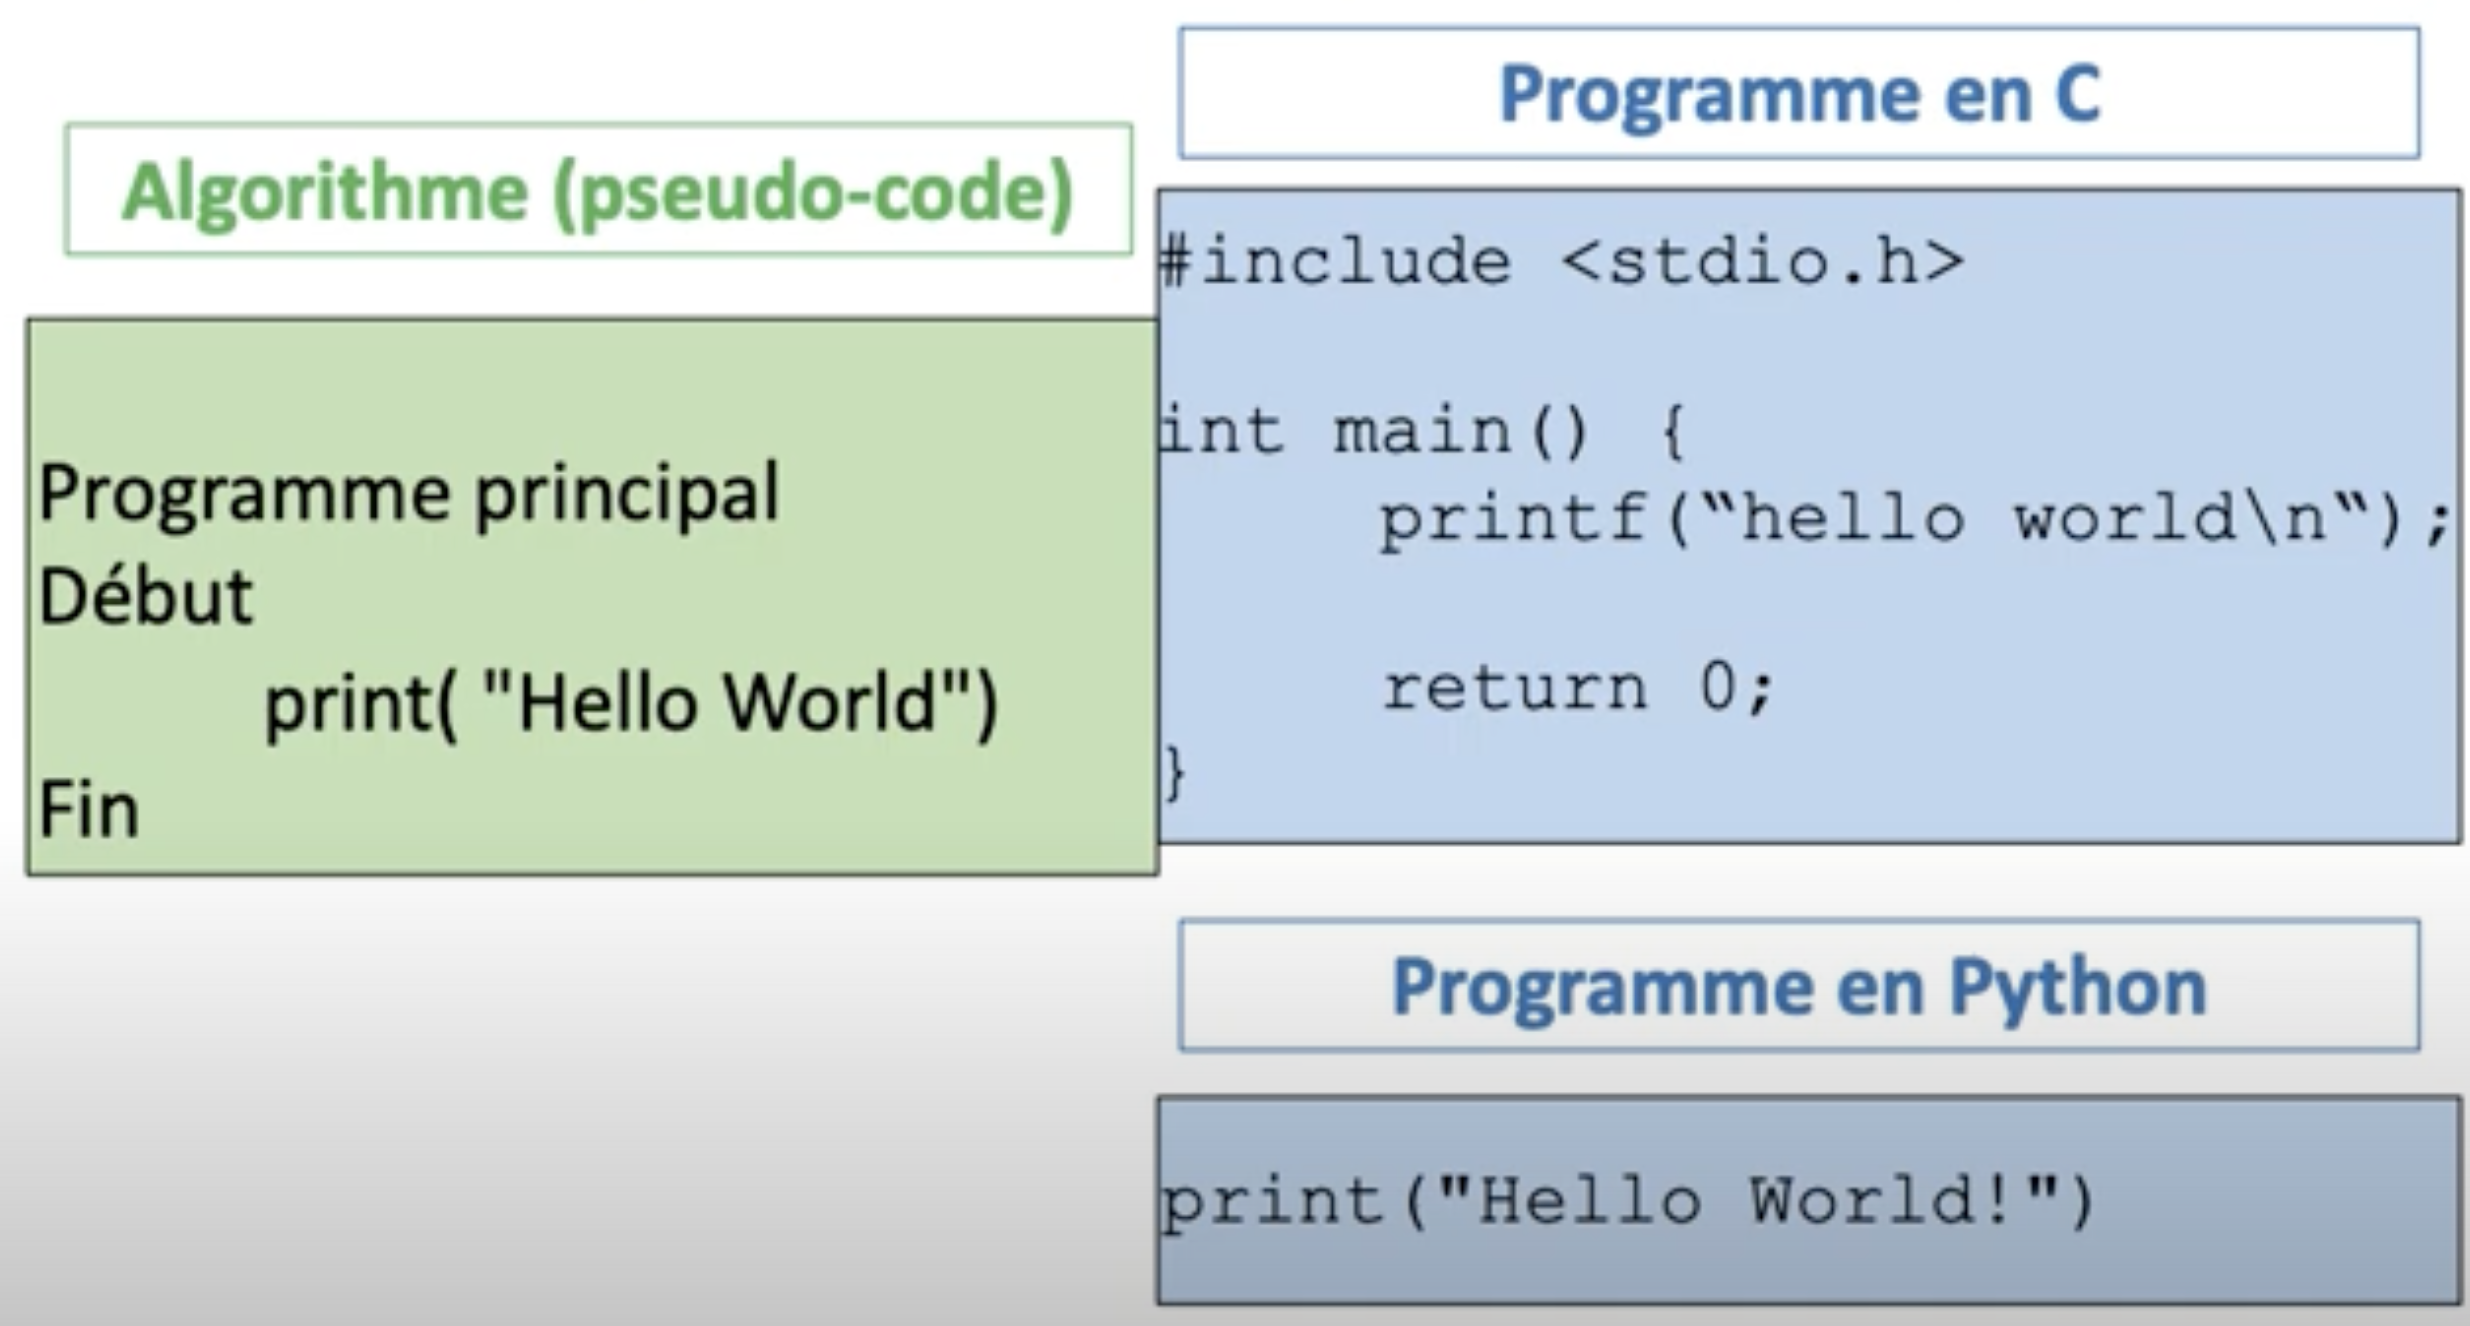
\includegraphics[width=0.5\textwidth]{001_AlgoHelloWorld.png}
		\end{figure}
		\item Conséquence: les règles de syntaxe de pseudo-code sont inspirées des éléments communs à la plupart des langages de programmation.
		\item Il n'y a pas de pseudo-code universel -- le seul principe à respecter, c'est que les règles de syntaxe appliquées soient bien définies, comprises et partagées par tous$\cdot$tes celles et ceux qui seront amené$\cdot$e$\cdot$s à lire les algorithmes.
	\end{alphenum}
	
	Ce dernier point implique qu'il y ait quand même une ossature de règles minimales dans un contexte donné -- comme pour ce cours par exemple:
	\begin{MaRgl}{pseudo-code en 1\textsuperscript{ère} NSI}
		\begin{alphenum}
			\item On spécifie explicitement en début d'algorithme les entrées attendues et les sorties prévues;
			\item On utilise une flèche vers la gauche ("$\leftarrow$" ou "$\lhd$") pour affecter des variables;
			\item On utilise l'indentation pour délimiter les fonctions, les conditions, les boucles...\footnote{Ici on triche un peu puisque l'indentation est spécifique à Python -- mais pas tant que ça puisque cela restera compréhensible même pour une implémentation dans un autre langage.}
			\item On explicite la fin de toute structure (fonction, condition, boucle...) débutée;
			\item On n'hésite pas à inclure des commentaires pour expliquer les étapes -- et dans ce cas, on les préfixe d'une flèche vers la droite ("$\rightarrow$" ou "$\rhd$")
			\item ... et c'est tout!
		\end{alphenum}
	\end{MaRgl}
	
	Pour illustrer ces principes, voici le pseudo-code d'une fonction (qu'on a déjà vue dans un chapitre précédent, d'ailleurs) prenant une liste de réels positifs en entrée et qui en renvoie le maximum:
	
	\vspace{\baselineskip}
	
	\begin{algorithmic}[1]
		\Require{$liste$ dont tous les éléments $\in \mathds{R+}$}
		\Ensure{$Max \in \mathds{R+}$}
		\Function{TrouveMax}{liste}
		\State Max $\leftarrow$ 0
		\ForAll{$Element$ de liste}
		\If{$Element > Max$}
		\Comment{On a trouvé un nouveau max}
		\State $Max$ $\leftarrow Element$
		\EndIf
		\EndFor
		\State\Return{$Max$}
		\EndFunction
	\end{algorithmic}
	
		\begin{MonExo}[Rédaction d'algorithmes en pseudo-code]
		En appliquant les principes énoncés ci-dessus, rédigez les algorithmes suivants:
		\begin{alphenum}
			\item Un algorithme qui prend deux nombres en entrée et affiche leur somme.
			\item Un algorithme qui calcule la somme des N premiers entiers naturels.
			\item Un algorithme qui génère les N premiers termes de la séquence de Fibonacci. (rappel: c'est une suite de nombres dont les deux premiers sont 0 et 1 et dont chaque élément est la somme des deux précédents -- donc: 0, 1, 1, 2, 3, 5, 8, 13, etc...).
			\item Un algorithme qui vérifie si une chaîne de caractères est un palindrome (se lit de la même manière dans les deux sens).
		\end{alphenum}
	\end{MonExo}
	
	\begin{MaReponse}
		Il n'y a jamais (ou rarement) une solution algorithmique unique à un problème -- ce qui suit n'est donc que des propositions de solution (qui sont, évidemment, valides -- mais pas uniques).
		\begin{alphenum}
			\item
			\begin{algorithmic}[1]
				\Require{deux nombres $a$ et $b$ $\in \mathds{R}$}
				\Ensure{$a + b$}
				\Function{Somme}{a, b}
				\State Resultat $\leftarrow$ a + b
				\State Afficher {$Resultat$}
				\EndFunction
			\end{algorithmic}
			\vspace{\baselineskip}
			\item
			\begin{algorithmic}[1]
				\Require{$N$ $\in \mathds{N}$}
				\Ensure{la somme des N premiers entiers naturels}
				\Function{SommeEntiers}{N}
				\State $Resultat$ $\leftarrow$ 0
				\Comment{On  initialise le résultat à 0}
				\For{$i$ allant de 0 à N}
				\State $Resultat$ $\leftarrow Resultat + i$
				\EndFor
				\State\Return{$Resultat$}
				\EndFunction
			\end{algorithmic}
			\vspace{\baselineskip}
			\item
			\begin{algorithmic}[1]
				\Require{$N$ $\in \mathds{N}$ avec $N > 2$}
				\Comment{On précise bien les valeurs acceptables en entrée}
				\Ensure{Liste des N premiers termes de la Suite de Fibonacci}
				\Function{Fibonacci}{N}
				\State Resultat $\leftarrow$ [0,1]
				\Comment{On initialise avec les deux premiers termes}
				\For{$i$ allant de 2 à N-1}
				\Comment{N premiers termes, donc on s'arrête à N-1}
				\State$Resultat[i] \leftarrow Resultat[i-1] + Resultat[i-2]$
				\EndFor
				\State\Return{Resultat}
				\EndFunction
			\end{algorithmic}
			\vspace{\baselineskip}
			\item
			\begin{algorithmic}[1]
				\Require{chn, une chaine de caractères}
				\Ensure{$Vrai$ ou $Faux$ selon si la chaine est un palindrome ou non}
				\Function{EstPalindrome}{chn}
				\State $Long$ $\leftarrow$ $longueur(chn)$
				\If{$Long$ est pair}
				\State $Milieu$ $\leftarrow$ $Long / 2$
				\Else
				\State $Milieu$ $\leftarrow$ $(Long  - 1) / 2$
				\EndIf
				\For{$i$ allant de 0 à Milieu}
				\If{$chn[i] \neq chn[Long - i]$}
				\State\Return{$Faux$}
				\EndIf
				\EndFor
				\State\Return{$Vrai$}
				\EndFunction
			\end{algorithmic}
			Quelques remarques sur cet algorithme:
			\begin{itemize}
				\item Lignes 8 et 9: le but ici est de bien comprendre l'algorithme -- avec cette formule on comprend bien ce qu'on fait: on part du début pour aller jusqu'au milieu. Strictement parlant les formules ne marchent pas (en Python chn[Long] donnerait une erreur) -- mais on s'en fiche: la démarche est claire ici, et c'est le but.
				\item Ligne 3: on vérifie la parité de la longueur puisque dans le cas des longueurs impaires on ignorera le caractère du milieu. Vous noterez qu'on dit ici "si Long est pair" sans expliquer comment on fait -- la difficulté de l'algorithme n'étant pas là, c'est tout à fait acceptable (on imagine qu'il y aura un algorithme pour une fonction "EstPair" explicité ailleurs).
				\item Lignes 10 et 13: c'est une démarche qu'on a déjà utilisée ailleurs pendant notre cours, qui est très classique, et qu'il faut impérativement maîtriser: on part du principe que quelque chose est vrai --- ici "chaîne est un palindrome" --- et dès qu'on trouve une preuve du contraire (ici: un caractère est différent de son homologue de l'autre côté) on retourne "Faux", c'est-à-dire qu'on arrête immédiatement la fonction puisqu'on connaît son résultat. Si on arrive au bout de la boucle, c'est qu'on a pas trouvé de preuve que c'est faux -- donc c'est vrai et c'est ce qu'on retourne.
			\end{itemize}
		\end{alphenum}
	\end{MaReponse}
	
	\begin{MonExo}[Traduction de pseudo-code en Python]
		\begin{alphenum}
			\item Traduisez en une fonction Python l'algorithme de la suite de Fibonacci;
			\item Traduisez en une fonction Python l'algorithme de vérification qu'un mot est un palindrome;
			\item \textbf{Expliquez comment vous allez tester votre fonction. Comment choisissez-vous les cas que vous allez tester?}
		\end{alphenum}
		\vspace{\baselineskip}
		Pensez bien à remplir correctement la documentation (ou docstring) de votre fonction. Que renvoie la fonction \texttt{help(nom\_de\_votre\_fonction)}?
	\end{MonExo}
	
	\begin{MaReponse}
		Pour la suite de Fibonacci, on pourra utiliser le code suivant:
		\MonPython{004_Fibonacci.py}
		Pour la tester, il suffira de la lancer avec différentes valeurs de N et de vérifier que le résultat est correct. Assez rapidement on constatera que si l'on passe une valeur de N qui n'est pas dans le champ des possibles (1, par exemple, ou -2) alors on obtient un résultat faux -- nous reviendrons plus tard dans ce cours sur comment gérer cela.
		\vspace{\baselineskip}
		
		Pour le palindrome, on pourra utiliser le code suivant:
		\MonPython{005_Palindrome.py}
		Pour la tester, il faudra réfléchir un peu plus à tous les cas de figures possibles:
		\begin{itemize}
			\item Chaine de longueur paire qui est un palindrome;
			\item Chaine de longueur paire qui n'en est pas un;
			\item Chaine de longueur impaire qui est un palindrome;
			\item Chaine de longueur impaire qui n'en est pas un.
		\end{itemize}
		
		Le choix des données à tester (les "jeux de tests") fait l'objet de la section suivante de ce cours.
		
		Vous aurez remarqué que la fonction help affiche à l'écran la docstring de la fonction que vous avez programmée -- utile, vous ne pensez pas?
	\end{MaReponse}
	
	\begin{MonRet}
		De cette section il faut que vous reteniez:
		\begin{itemize}
			\item Les éléments qu'il faut systématiquement inclure dans la rédaction du pseudo-code d'une fonction:
			\begin{itemize}
				\item Ses entrées -- et conditions qui s'y appliquent;
				\item Ses sorties;
				\item Le traitement des données.
			\end{itemize}
			\item Les \textit{principes} de rédaction de pseudo-code -- et par-dessus tout \textbf{le fait que le pseudo-code ne peut pas souffrir d'ambiguïté}. Le plus simple pour atteindre cet objectif est de commencer par se conformer aux règles énoncées ici;
			\item Ne pas perdre de vue que la traduction d'un algorithme en code Python est un exercice en soi: la \textit{logique} de la démarche appartient à l'algorithme, mais son \textit{implémentation} relève du bon usage de la syntaxe du langage.
		\end{itemize}
	\end{MonRet}
	
	\subsection{Tester un algorithme}
	
	Cette étape est cruciale dans le développement d'un programme informatique car les erreurs dans les phases de rédaction de l'algorithme et de traduction en langage de programmation sont plus que fréquentes -- elles sont systématiques dès lors qu'un programme atteint un certain niveau de complexité.
	
	Un test permet de vérifier que l'algorithme fonctionne sur une donnée précise. Pour programmer efficacement il faut concevoir des \textit{jeux de tests} permettant de vérifier que l’algorithme renvoie, dans des cas particuliers bien choisis, ce que l’on attend de lui. Il est impossible d'écrire un ensemble de tests permettant d’exclure toutes les erreurs possibles, mais on peut cependant essayer d'en construire un en respectant déjà les règles suivantes:
	
	\begin{MaRgl}{tester une fonction}
			 Les \textbf{jeux de tests} (ensembles de données que l'on va tester) à préparer pour tester une fonction donnée doivent:
			 \begin{itemize}
			 	\item Si la spécification de l'algorithme mentionne plusieurs cas possibles, les tester tous (ex: chaines de caractères paires et impaires pour le palindrome);
			 	\item Si l'algorithme doit renvoyer une valeur booléenne, construire des tests permettant d’obtenir les deux valeurs de vérité (toujours l'exemple du test de palindrome);
			 	\item Si l'algorithme s'applique à une liste / un tableau, effectuer un test avec un tableau vide;
			 	\item Si l'algorithme s'applique à un nombre, effectuer des tests avec des valeurs positives, négatives, et avec zéro.
			 \end{itemize}
			 \vspace{\baselineskip}
			 
			Attention: ces règles ne sont pas exhaustives -- vous devez plus les voir comme des principes à appliquer et à adapter à chaque fonction que vous développez.
	\end{MaRgl}
	
	\begin{MonRet}
		 	\textbf{Apprendre par cœur les règles énoncées ici n'aurait aucun sens.} Ce qu'il faut comprendre ce sont les principes qui les sous-tendent et être capable, pour les fonctions que vous allez développer (en exercice, projet, ou contrôle), de proposer des jeux de tests qui les respectent.
	\end{MonRet}
	
	\pagebreak
	\section{Preuves d'algorithmes}
	On vient de voir comment tester un algorithme -- démarche qui va nous permettre de nous rendre compte, sur des cas concrets, s'il se comporte de la manière que l'on souhaite. On ne peut en revanche jamais tester \textit{l'intégralité} des situations possibles, et il est parfois vital d'être certain, malgré cela, que l'algorithme se termine et produit le résultat attendu à tous les coups -- on peut penser par exemple à l'informatique embarquée dans le pilotage automatique de voitures ou de trains...
	
	Pour atteindre ce but on va (comme on le ferait en mathématiques) \textbf{\textit{démontrer}} qu'un algorithme est correct, et ce en deux étapes:
	\begin{itemize}
		\item La \textbf{\textit{terminaison}}: on montre que l'algorithme se termine.
		\item La \textbf{\textit{correction partielle}}: on montre que l'algorithme produit bien le résultat attendu.
	\end{itemize}
	
	\subsection{Terminaison: variant de boucle}
	Dans ce cours on va limiter le champ de cette étude à la vérification que toute boucle \texttt{tant que} (ou boucle conditionnelle, ou boucle \texttt{while}) se termine bien et n'est pas infinie. En effet, dans le contexte du programme de 1\textsuperscript{ère}, c'est le seul cas où la terminaison ne serait pas garantie puisque, d'une part, les seules structures se répétant que nous envisageons sont les boucles\footnote{En terminale on s'intéressera à la récursivité qui induisent des répétitions potentiellement infinies sans l'utilisation de boucles.}, et que, d'autre part, les boucles \texttt{pour} (ou boucles itératives, ou boucles \texttt{for}) sont conçues pour se terminer au bout d'un nombre d'itérations donné, fixé, et connu à l'avance\footnote{même si on peut en théorie imaginer une boucle allant "de 1 à n" dans laquelle on augmente n... Mais c'est en dehors du périmètre de ce cours.}.
	
	Pour prouver qu’un algorithme s'arrête, il faut donc démontrer que pour chaque boucle \texttt{tant que}, la condition d'entrée \textbf{sera invalidée dans un temps fini} -- ou, dit autrement, après un nombre fini de passages dans cette boucle. La plupart du temps, cela revient à montrer qu'il existe un \textbf{variant} pour chacune de ces boucles.
	
	\begin{MaDef}{variant de boucle}
		Un \textbf{variant de boucle} est une quantité entière positive qui décroît strictement à chaque itération de la boucle (une suite d’entiers naturels strictement décroissante est nécessairement finie).
		\vspace{\baselineskip}
		
		Exemple, pour la boucle suivante, on peut aisément se convaincre que la quantité $5 - i$ est un variant de boucle selon la définition ci-dessus: elle commence à 5 puis décroît jusqu'à atteindre 0 -- on est donc bien certains que la boucle se terminera.
		
		\begin{algorithmic}[1]
			\State i $\leftarrow$ 0
			\While{i < 5}
			\State i $\leftarrow$ i + 1
			\EndWhile
		\end{algorithmic}
	\end{MaDef}
	
		Attention! Pour qu'une quantité soit un variant de boucle il faut bien qu'elle décroisse, \textbf{\textit{mais aussi}} qu'elle soit \textbf{\textit{toujours}} positive -- en d'autres termes que la condition d'arrêt de la boucle ne soit pas étroite au point de permettre au variant de "dépasser" 0. Considérez la boucle suivante par exemple:
	\begin{algorithmic}[1]
		\State i $\leftarrow$ 0
		\State\While{$i \neq 5$}
		\State i $\leftarrow$ i + 2
		\EndWhile
	\end{algorithmic}
	
	On voir bien que dans ce cas $5-i$ décroît bien... mais devient assez rapidement négatif!
	
	\begin{MonExo}[Variant de boucle]
		Considérez les deux algorithmes suivants:
		\vspace{\baselineskip}
		
		\begin{tabular}{p{0.5\textwidth}p{0.5\textwidth}}
			\begin{minipage}{\linewidth}
				\begin{algorithmic}[1]
					\State Afficher "entrez un entier positif"
					\State lire $Nb$
					\State i $\leftarrow$ 0
					\While{$Nb > 0$}
					\State $Nb \leftarrow Nb$ // $10$
					\State i $\leftarrow$ i + 1
					\EndWhile
					\State Afficher i
				\end{algorithmic}
			\end{minipage}
		&
			\begin{minipage}{\linewidth}
				\begin{algorithmic}[1]
					\State Afficher "entrez un entier positif"
			 		\State lire $Nb$
			 		\State $k \leftarrow 1$
			 		\State $i \leftarrow 0$
			 		\While{$k < (Nb + 1)$}
			 		\State $k \leftarrow k \times 10$
			 		\State $i \leftarrow i + 1$
			 		\EndWhile
			 		\State Afficher i
			 	\end{algorithmic}
			 \end{minipage}
		\\
		\end{tabular}
		\vspace{\baselineskip}
		
		\begin{alphenum}
			\item Que sont censés faire ces algorithmes?
			\item Utilisez la technique du variant pour justifier que le premier se termine.
			\item Que se passerait-il si on remplaçait la condition "$Nb > 0$" par "$Nb \neq 0$"?
			\item Utilisez la technique du variant pour justifier que le second se termine.
			\item Que se passerait-il si on remplaçait "$k < (Nb + 1)$" par "$k \neq (Nb + 1)$"?
		\end{alphenum}
	\end{MonExo}
	\begin{MaReponse}
		\begin{alphenum}
			\item Les deux sont censés afficher le nombre de chiffres que comporte le nombre entré par l'utilisateur:
			\begin{itemize}
				\item Le premier effectue des divisions entières successives du nombre jusqu'à atteindre 0;
				\item Le second procède "dans l'autre sens" en partant de 1 et en multipliant par 10 jusqu'à dépasser le nombre.
			\end{itemize}
			\item Le variant ici est le nombre $Nb$: en effet, pour tout nombre strictement positif, sa division entière par 10 lui est strictement inférieure -- $Nb // 10 < Nb$; donc $Nb$ est strictement décroissant.
			\item Si l'on remplace "$Nb > 0$" par "$Nb \neq 0$" le variant demeure valide. En effet, à terme, les divisions entières successives par 10 atteignent exactement 0 (et ne peuvent en aucun cas devenir négatives).
			\item Le variant ici est la quantité $Nb + 1 - k$ -- il est facile de se convaincre qu'à chaque itération de la boucle, k étant multiplié par 10, la quantité décroît strictement.
			\item Si on remplaçait "$k < (Nb + 1)$" par "$k \neq (Nb + 1)$" en revanche, l'arrêt n'aurait plus lieu que pour les valeurs de Nb égales à 9, 99, 999, etc... -- pour toutes les autres, le variant passera en négatif sans "s'arrêter" à la valeur 0.
		\end{alphenum}
	\end{MaReponse}
	
	\begin{MonRet}
		De cette section il faut évidemment avoir compris ce qu'est un variant de boucle, mais il faut surtout être capable de résoudre des exercices tel que celui ci-dessus: \textbf{identifier} le variant de boucle, \textbf{prouver} qu'il décroît strictement, en \textbf{déduire} en appliquant la condition de la boucle qu'elle se termine.
	\end{MonRet}
	
	\subsection{Correction partielle: invariant de boucle}
	On va s'intéresser ici (dans le cadre du programme de 1\textsuperscript{ère}) à démontrer la correction des boucles dont on conçoit les algorithmes et, pour ce faire, on va se poser des questions du type:
	\begin{itemize}
		\item Les variables sont-elles bien initialisées \textit{avant} le début de la boucle?
		\item Le nombre de tours de la boucle est-il correct?
		\item S'il y en a un, est-ce que l'indice est bien choisi?
		\item Et, \textit{in fine}, les valeurs obtenues en sortie de boucle sont-elles les bonnes?
	\end{itemize}
	
	Toutes ces questions vont être abordées au moyen de la notion d'\textit{invariant de boucle}.
	
	\begin{MaDef}{invariant}
		Un \textbf{invariant} est une propriété d'un algorithme qui reste vraie tout au long de son exécution.
	\end{MaDef}
	
	Un invariant de boucle est une proposition toujours vraie à chaque fois que l'on entre dans la boucle. La démarche que nous allons adopter se déroule en quatre étapes:
	\begin{enumerate}
		\item On choisit l'invariant:
		\begin{itemize}
			\item Comprendre clairement le but de la boucle -- qu'est-elle censée accomplir? Quel est le résultat attendu?
			\item Partir "de la fin", c'est-à-dire du résultat attendu et identifier quelle quantité est "construite" au fur et à mesure des itérations de la boucle pour constituer ce résultat.
			\item Ceci devrait vous mettre sur la voie de votre invariant -- une propriété (somme d'éléments déjà traités, ordre d'éléments dans une liste...) qui ne change pas malgré les itérations de la boucle.
			\end{itemize}
		\item On montre que l’invariant est vérifié avant la boucle (initialisation);
		\item On montre que si l'invariant est vérifié \textit{avant }un passage dans la boucle, alors il est préservé \textit{après }le passage dans la boucle;
		\item On peut conclure sur la valeur finale à la sortie de la boucle.
	\end{enumerate}
	
	Et ainsi, \textit{par récurrence}, on démontre la correction partielle.
	
	$\rhd$ Ca vous semble très abstrait? Vous avez notamment l'impression que le choix de l'invariant est \textit{très, très, très} flou? C'est normal! Le seul moyen d'expliquer ça clairement est de s'appuyer sur des exemples...
	
	Considérons la fonction suivante:
	\begin{algorithmic}[1]
		\Require{$a, b$ $\in \mathds{N}$ avec}
		\Ensure{Le produit $a \times b$}
		\Function{Produit}{a, b}
		\State m $\leftarrow$ 0
		\State p $\leftarrow$ 0
		\While{$m < a$}
		\State m $\leftarrow$ m + 1
		\State p $\leftarrow$ p + b
		\EndWhile
		\State\Return{p}
		\EndFunction
	\end{algorithmic}
	
	On commence par noter qu'on a bien un variant de boucle... Lequel?\footnote{$a - m$ bien sûr!} La terminaison est donc prouvée.
	
	Etapes de la démarche:
	\begin{enumerate}
		\item Choix de l'invariant: le but est de renvoyer le produit p qui, à la fin, vaudra $a \times b$; il est construit dans cette boucle par ajouts successifs de $b$, $m$ fois. On peut donc avoir l'intuition que l'invariant est $p = m \times b$. Vérifions cela avec les deux étapes suivantes.
		\item Avant la boucle on a $p$ et $m$ tous les deux à 0 -- donc l'invariant est vérifié.
		\item Supposons qu'au début d'une itération de la boucle l'invariant est vérifié, avec m et p; à la fin de cette itération, les valeurs respectives de m et p seront de $m' = m + 1$ et $p' = p + b$.  On aura alors:
		\[ p' = p + b = m \times b + b = (m + 1) \times b = m' \times b\]
		Et donc l'invariant est bien vérifié à la fin de la boucle.
		\item En fin de boucle on a $m = a$ et donc à la sortie de la boucle on a bien $p = a \times b$.
	\end{enumerate}
	
	On a donc bien démontré la correction de la boucle.
	
	\begin{MonExo}[Détermination d'un invariant de boucle]
		Donner un invariant de boucle pour la fonction suivante qui calcule x à la puissance n:
		\begin{algorithmic}[1]
			\Require{$x, n \in \mathds{N}$}
			\Ensure{$x^n$}
			\Function{Puissance}{x, n}
			\State r $\leftarrow$ 1
			\For{i allant de 0 à n - 1}
			\State $r \leftarrow r \times x$
			\EndFor
			\State\Return{r}
			\EndFunction
		\end{algorithmic}
	\end{MonExo}
	
	\begin{MaReponse}
		La démarche est extrêmement proche de celle qu'on a adoptée pour le produit dans l'exemple précédent:
		\begin{enumerate}
			\item On peut choisir comme invariant "$r = x^i$";
			\item Au début de la boucle on a $r = 1$ et $i = 0$, donc l'invariant $r = x^i$ est bien vérifié, quel que soit x.
			\item Si au début d'une itération de la boucle on a l'invariant vérifié, notons $r' = r \times x$ et $i' = i + 1$ les valeurs respectives de r et i à la fin de cette itération. On a:
			\[ r' = r \times x = x^i \times x = x^{i+1} = x^{i'}\]
			\item En fin de boucle on est passé $n$ fois dans la boucle (de 0 à (n-1)) donc on a bien $r = x^n$.
		\end{enumerate}
	\end{MaReponse}

	Un invariant de boucle peut être une formule mathématique (une égalité, une inégalité) mais pas nécessairement -- il peut également être une \textit{propriété} qui reste vraie tout au long de la boucle. 
	
	\begin{MonExo}[Un autre invariant d'un type un peu différent]
		Considérez le code suivant:
		\MonPython{006_ListeNbPairs.py}
		
		\begin{alphenum}
			\item La docstring semble effacée et le nom de la fonction incomplet -- que fait cette fonction selon vous?
			\item Quel est le variant de boucle?
			\item Quel est la propriété (portant sur les nombres de la liste et faisant intervenir l'indice \texttt{i}) qui constitue l'invariant de boucle de cette fonction?
		\end{alphenum}
	\end{MonExo}
	
	\begin{MaReponse}
		\begin{alphenum}
			\item On se convainc assez facilement que la fonction cherche à vérifier si tous les nombres de la liste passée en entrée sont pairs. Mais si on n'en est pas convaincu, on peut le prouver -- c'est tout l'intérêt des invariants de boucle!
			\item Le variant de boucle est à l'évidence $len(liste) - i$ -- je vous laisse le démontrer. A noter que la condition \texttt{liste[i] \% 2 == 0} ne change rien à la preuve de terminaison puisque tout ce qu'elle pourra changer sera que la boucle se termine \textit{avant} que le variant n'atteigne 0.
			\item Démarche pour l'invariant de boucle:
			\begin{enumerate}
				\item Choix de l'invariant: le but est de une évaluation de si tous les nombres de la liste sont pairs. L'invariant va donc nécessairement avoir quelque chose à voir avec une liste de nombre pairs (sinon il ne permettra pas de prouver la correction partielle de la boucle et donc ne servira à rien). En creusant un peu on arrive à constater qu'à tout moment, en théorie, tous les nombres qui ont été passés en revue par la boucle sont pairs (car sinon on sort de la boucle). On peut donc exprimer l'invariant comme étant la propriété P(i) suivante: "Pour tout indice k de 0 à i-1, liste[k] \% 2 == 0".
				\item Il est vrai avant la première itération de la boucle -- puisqu'on n'a vérifié aucun nombre à cette étape, la propriété est vraie.
				\item S'il est vrai avant d'incrémenter i, la condition de la boucle donne deux résultats possibles:
				\begin{itemize}
					\item Si cette condition est vraie, alors P(i) reste vrai pour la prochaine valeur de i.
					\item Si la condition n'est pas vraie, la boucle s'arrête et on ne touche plus à i.
				\end{itemize}
				\item De la même manière, lorsque la boucle se termine, c'est pour une de deux raisons:
				\begin{itemize}
					\item C'est soit parce que i est égal à len(liste), et dans ce cas tous les éléments sont pairs -- puisqu'on a bien considéré tous les éléments de la liste, de 0 à \texttt{len(liste) - 1} -- et P(i) est vrai, ce qui signifie que la fonction retourne True,
					\item Ou parce qu'on a trouvé un élément impair et dans ce cas la boucle s'arrête et P(i) indique que tous les éléments avant cet indice sont pairs, mais pas l'élément à l'indice i, donc la fonction retourne False.
				\end{itemize}
			\end{enumerate}
		\end{alphenum}
	\end{MaReponse}
	
	\begin{MonExo}[Et un dernier pour la route...]
		Montrer que $r = a - b \times q$ est bien un invariant de boucle de la fonction suivante, qui réalise une division euclidienne:
		\begin{algorithmic}[1]
			\Require{$a, b \in \mathds{N}; b\neq 0$}
			\Ensure{$q, r$ le quotient et le reste de la division euclidienne de a par b}
			\Function{DivEuclid}{a, b}
			\State r $\leftarrow$ a
			\State q $\leftarrow$ 0
			\While{$r \geq b$}
			\State $r \leftarrow r - b$
			\State $q \leftarrow q + 1$
			\EndWhile
			\State\Return{q, r}
			\EndFunction
		\end{algorithmic}
	\end{MonExo}
	
	\begin{MaReponse}
		La démarche est extrêmement proche de celle qu'on a adoptée pour le produit dans l'exemple précédent:
		\begin{enumerate}
			\item Le choix de la quantité identifiée comme invariant est donné par l'énoncé;
			\item Au début de la boucle on a $r = a$ et $q = 0$, donc l'invariant $r = a - b \times q$ est bien vérifié, quel que soit b.
			\item Si au début d'une itération de la boucle on a l'invariant vérifié, notons $r' = r - b$ et $q' = q + 1$ les valeurs respectives de r et q à la fin de cette itération. On a:
			\[ r' = r - b = a - b \times q - b = a - b \times (q + 1) = a - b \times q'\]
			\item En fin de boucle l'invariant est nécessairement encore vrai, par récurrence (le point 2 ci-dessous étant l'initialisation et le point 3 la preuve de la récurrence).
		\end{enumerate}
	\end{MaReponse}
		
	\begin{MonRet}
		Ce qu'il faut retenir de cette section est l'équivalent de ce qui était nécessaire pour la précédente:
		\begin{itemize}
			\item Comprendre la notion d'invariant de boucle;
			\item Être capable de résoudre des exercices comme ceux ci-dessus: \textbf{identifier} un invariant de boucle, \textbf{montrer} qu'il est vrai \textbf{avant la boucle}, \textbf{prouver par récurrence} qu'il l'est à toutes les itérations de la boucle, et en \textbf{déduire la correction partielle }de la boucle.
		\end{itemize}
		Note: je vous fournirai prochainement un cahier d'exercices corrigés pour vous entrainer sur les invariants, les variants --- et plus généralement sur tout le contenu de ce chapitre.
	\end{MonRet}
	
	\pagebreak
	\section{Complexité d'algorithmes}
	\subsection{Cadre théorique}
	Lorsque l'on commence à traiter d'importants volumes de données, que l'on commence à considérer des traitements complexes, ou tout simplement longs en nombre d'instructions exécutées se pose la question de la \textit{performance} du traitement. On évalue cette performance suivant deux axes:
	\begin{itemize}
		\item \textbf{Performance temporelle} (que nous allons aborder ici) -- il s'agit du temps d'exécution du programme.
		\item \textbf{Performance spatiale }(qui n'est pas au programme) -- il s'agit de la mémoire nécessaire à l'exécution du programme (pour stocker notamment l'intégralité des variables qu'il manipule).
	\end{itemize}
	
	On ne s'intéresse pas ici à la durée exacte d'exécution d'un programme -- celle-ci est trop dépendante de la machine sur laquelle on l'exécute, des autres traitements en cours le cas échéant, du langage de programmation... Ce à quoi on va s'intéresser c'est à la mesure du \textbf{nombre d'opérations élémentaires} que va effectuer un programme en fonction des données qu'il va recevoir en entrée. Par "opération élémentaire" on entend "étape" du programme (ligne de code, le plus souvent) dont, pour simplifier, on va considérer qu'elles prennent toutes la même temps à exécuter. Ainsi, en estimant grossièrement le nombre d'opérations élémentaires en fonction du volume de données en entrée on pourra commencer à se faire une idée de la performance d'un algorithme donné: c'est ce qu'on appelle un \textbf{calcul de complexité}.
	
	Le but principal d'un calcul de complexité est de pouvoir comparer l’efficacité entre différents algorithmes répondant à un même problème. En d'autres termes, de répondre à la question: "\textit{Quelle que soit la machine et le langage de programmation utilisé, l'algorithme A est-il plus performant que l'algorithme B pour de grands volumes de donénes?}"
	
	\begin{MaDef}{complexité d'un algorithme}
		La \textbf{complexité d’un algorithme} est une mesure intrinsèque à l'algorithme qui est indépendante de toute implémentation. Elle est calculée en fonction d’un \textit{paramètre représentatif des entrées} (la taille) et à l'aide d'une \textit{mesure élémentaire} (nombre de comparaisons, nombre d’opérations arithmétiques, etc.).
	\end{MaDef}
	
	\subsection{Exercices d'application}
	Le plus simple pour comprendre ces notions est de démarrer par quelques exemples concrets -- on en déduira à la section suivantes des règles et une méthode d'évaluation de la complexité.
	\begin{MonExo}[Comptage d'opérations élémentaires]
		Pour chacun des deux algorithmes suivants, calculer le nombre d'opérations élémentaires effectué. Dépend-il des données en entrée?
		
		\begin{tabular}{p{0.5\textwidth}p{0.5\textwidth}}
			\begin{minipage}{\linewidth}
				\begin{algorithmic}[1]
					\Function{Produit1}{n, b}
					\State p $\leftarrow n \times b$
					\State\Return{p}
					\EndFunction
				\end{algorithmic}
			\end{minipage}
			&
			\begin{minipage}{\linewidth}
				\begin{algorithmic}[1]
					\Function{Produit2}{n, b}
					\State m $\leftarrow$ 0
					\State p $\leftarrow$ 0
					\While{$m < n$}
					\State m $\leftarrow$ m + 1
					\State p $\leftarrow$ p + b
					\EndWhile
					\State\Return{p}
					\EndFunction
				\end{algorithmic}
			\end{minipage}
			\\
		\end{tabular}
	\end{MonExo}
		
	\begin{MaReponse}
		Pour Produit1, c'est vite vu: 2 opérations (le produit et le "retourner") quelles que soient les données en entrée.
		
		Pour Produit2 c'est un peu plus compliqué:
		\begin{itemize}
			\item On a trois opérations effectuées quoi qu'il arrive (les deux affectations avant la boucle, et le "retourner").
			\item Dans la boucle, on a deux opérations également: le calcul du nouveau m et le calcul du nouveau p.
			\item On a également une opération "cachée" dans la boucle: la comparaison "$m < n$" qui doit être effectuée à chaque itération -- ce qui nous fait un total de trois opérations pour la boucle.
			\item La boucle est effectuée $n$ fois --- de $m = 0$ à $m = n - 1$.
			\item Le nombre total d'opérations élémentaires pour Produit2 est donc de: $3 \times n + 2$ (il dépend donc de la valeur de n uniquement -- pas de celle de b).
		\end{itemize}
		
		Je vous laisse deviner lequel de ces deux algorithmes est le meilleur pour déterminer le produit de deux entiers n et b (imaginez le calcul de 10 milliards $\times 2$ par exemple).
			
	\end{MaReponse}

		\begin{MonExo}[Complexité -- somme des premiers entiers]
		Reprenons un algorithme qu'on avait écrit dans un exercice précédent et qui calculait la somme des n premiers entiers:
		
		\begin{algorithmic}
			\Require{$n$ $\in \mathds{N}$}
			\Ensure{la somme des N premiers entiers naturels}
			\Function{SommeEntiers}{N}
			\State $Resultat$ $\leftarrow$ 0
			\For{$i$ allant de 1 à N}
			\State $Resultat$ $\leftarrow Resultat + i$
			\EndFor
			\State\Return{$Resultat$}
			\EndFunction
		\end{algorithmic}
		\vspace{\baselineskip}
		Quelle est sa complexité?\footnote{Derrière cette question s'en cachent en fait deux: 1/ combien d'opérations élémentaires effectue l'algorithme? 2/ de quelle quantité ("paramètre représentatif des entrées") dépend ce nombre et selon quelle formule mathématique?}
	\end{MonExo}
	
	\begin{MaReponse}
		\begin{itemize}
			\item On a deux opérations en-dehors de la boucle (que l'on va assez rapidement apprendre à ignorer -- il est évident qu'elles n'ont aucune influence sur la performance globale de l'algorithme).
			\item On a une opération évidente dans la boucle: l'ajout de l'entier en cours au résultat.
			\item On a en fait deux opérations cachées en plus: l'incrémentation de i, d'une part, et sa comparaison avec n d'autre part.
		\end{itemize}
		
		On arrive donc à un total de $3 \times n + 2$ opérations élémentaires -- on peut donc dire que la complexité de l'algorithme \textbf{dépend de n}.\footnote{Pour prouver que les maths sont parfois utiles: on sait que $1 + 2 + ... + n = \frac{n(n + 1)}{2}$. Il est donc possible de faire le même calcul en exactement quatre opérations contre plus de 3 millions par exemple si on utilise l'algorithme de l'énoncé sur les un million premiers entiers...}
	\end{MaReponse}
	
	\begin{MonExo}[Complexité -- boucles imbriquées]
		Envisageons à présent la fonction suivante, qui contient deux boucles imbriquées, et pour laquelle la complexité sera un peu plus compliquée à estimer:
		\MonPython{Exos_008_CheckDupliq.py}
		\begin{alphenum}
			\item Quelle est sa complexité?
			\item (question bonus) Ne pensez-vous pas que cet algorithme effectue des opérations inutiles? Lesquelles? Comment l'améliorer?
		\end{alphenum}
	\end{MonExo}
	
	\begin{MaReponse}
		\begin{alphenum}
			\item Commençons par nous assurer que nous avons bien compris le fonctionnement de l'algorithme derrière cette fonction, en imaginant qu'on lui passe en entrée une liste de 5 lettres \texttt{['A', 'J', 'T', 'J', 'K']}:
			\begin{figure}[H]
				\centering
				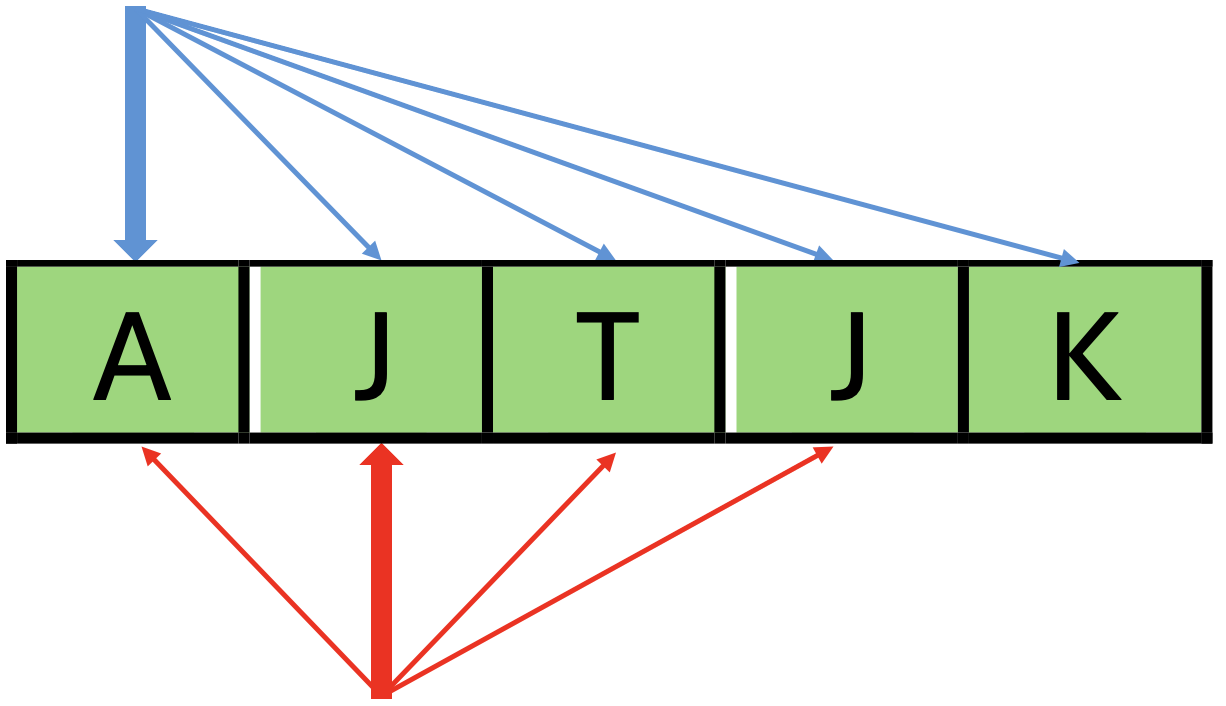
\includegraphics[width=0.5\textwidth]{004_ChercheDupliq.png}
			\end{figure}
			On a ici \textbf{\textit{deux boucles imbriquées}}:
			\begin{itemize}
				\item La boucle \textit{extérieure} (\texttt{for i in range(len(liste))}) est représentée sur le schéma par les flèches épaisses et verticales. Pour chaque valeur à l'intérieur de cette boucle, on exécute...
				\item ... la boucle \textit{intérieure} (\texttt{for j in range(len(liste))}) qui est représentée sur le schéma par les flèches fines et diagonales.
			\end{itemize}
			On se convainc facilement que dans ce cas les comparaisons représentées en bleu (A-J, A-T, A-J, A-K) seront effectuées en premier sans trouver de doublon, puis ce seront les comparaisons en rouge, (J-A, J-T, J-J) et la fonction s'arrêtera sur la dernière puisqu'on aura trouvé un doublon, et elle renverra True.
			
			Le nombre d'opérations élémentaires dépend donc à l'évidence de deux choses:
			\begin{itemize}
				\item La longueur \textbf{(qu'on va appeler "n")} de la liste en entrée;
				\item La présence et la localisation du premier doublon -- si la liste avait été ['J', 'J', 'A', 'T', 'K'] le traitement aurait immédiatement trouvé un doublon et donc n'aurait effectué qu'une comparaison, tandis que si la liste n'avait pas contenu de doublons l'intégralité des deux boucles aurait été parcourue.
			\end{itemize}
			Comme on va l'expliquer ci-dessous on va considérer la situation "au pire", c'est à dire celle où la complexité est la plus élevée, donc celle où la liste en entrée ne contient pas de doublon.
			
			Comme c'est décrit ci-dessus, la boucle \textit{intérieure} est exécutée intégralement pour chaque valeur de la boucle \textit{extérieure} -- pour déterminer le nombre total d'opérations élémentaires il nous suffit donc de calculer les nombre d'opérations de chacune de ces boucles et de les multiplier entre eux.
			\begin{itemize}
				\item La boucle extérieure est simple: elle effectue "n" incrémentations de j;
				\item La boucle intérieure effectue une incrémentation de i ainsi que deux comparaisons ("\texttt{i != j}" et "\texttt{liste[i] == liste[j]}"), et ce n fois.
			\end{itemize}
			
			On en conclut donc que, "au pire", la complexité de la fonction sera de $n \times (3 \times n) = 3n^2$.)
			
			\item Dans l'exemple, on peut constater que la comparaison entre A et le premier J est effectuée deux fois -- une fois quand la boucle extérieure est positionnée sur le A, et une autre fois quand elle l'est sur le J. C'est évidemment inutile, il suffirait de faire des comparaisons, dans la boucle intérieure, uniquement sur les éléments de la liste situés \textit{après} celui de la boucle extérieure, donc d'indice démarrant à (i+1):
			\MonPython{Exos_009_CheckDupliq_Optim.py}
			(et on notera au passage que grâce au démarrage de j à l'indice i+1 on s'évite également à chaque passage la comparaison \texttt{i != j} que l'on avait dans la version précédente de l'algorithme)
		\end{alphenum}
		
	\end{MaReponse}
	
	\subsection{Principes d'estimation de la complexité}
	
	Sur la base de ce que l'on vient de voir dans les exercices, on peut poser les principes de calcul de la complexité suivants:
	\begin{MaRgl}{Calcul de complexité}
		\begin{itemize}
			\item On commence par "compter" le nombre d'opérations élémentaires -- et en déduire le paramètre représentatif des entrées dont la complexité dépend (le plus souvent ce sera la longueur d'une liste ou d'une chaîne, la valeur d'un nombre...).
			\item On se place dans un contexte "au pire": lorsque plusieurs cas sont possibles on simplifie en considérant que le maximum possible d'opérations va être effectué.
			\item On se limite à l'\textit{ordre de grandeur} de la complexité -- en d'autres termes on ignore tous les termes du calcul que l'on vient de faire à l'exception de sa plus importante dépendance au paramètre des entrées: on ignore les valeurs constantes quand il y a une dépendance à n, les puissances de n inférieures à la plus grandes, les facteurs multiplicateurs constants... Exemples:
			\begin{itemize}
				\item Si notre calcul a donné $3n + 1$ on dira que l'ordre de grandeur de la complexité dépend de $n$, et on parlera d'une "complexité linéaire".
				\item Si notre calcul a donné $7n^2 + 3n + 1$ on dira que l'ordre de grandeur de la complexité dépend de $n^2$, et on parlera d'une "complexité quadratique".
				\item Cas particulier: si notre calcul a donné $5$ opérations, on dira que la complexité est constante (ne dépend pas des entrées).
			\end{itemize}
			\item Cette complexité est décrite en utilisant la notation "$\mathcal{O}$" (appelée "grand O") -- ainsi, pour les trois cas précédents on notera les complexités, respectivement, $\mathcal{O}(n)$ (complexité linéaire), $\mathcal{O}(n^2)$ (complexité quadratique), et $\mathcal{O}(1)$ (complexité constante).
		\end{itemize}
	\end{MaRgl}
	
	\begin{MonExo}[Nommons les complexités précédentes]
		En appliquant ces règles:
		\begin{alphenum}
			\item Comment peut-on nommer et noter les complexités des fonctions des exercices précédents -- \texttt{Produit1}, \texttt{Produit2}, \texttt{SommeEntiers}, et \texttt{Verif\_Doublons}?
			\item Est-ce que la complexité de la version optimisée de \texttt{Verif\_Doublons} (qu'on a appelée \texttt{Verif\_Doublons\_Optim}) serait différente de celle de \texttt{Verif\_Doublons}?
		\end{alphenum}
	\end{MonExo}
	
	\begin{MaReponse}
		\begin{alphenum}
			\item
			\begin{itemize}
				\item \texttt{Produit1} a une complexité constante ($\mathcal{O}(1)$);
				\item \texttt{Produit2} a une complexité linéaire ($\mathcal{O}(n)$);
				\item \texttt{SommeEntiers} a une complexité linéaire ($\mathcal{O}(n)$);
				\item \texttt{Verif\_Doublons} a une complexité quadratique ($\mathcal{O}(n^2)$).
			\end{itemize}
			\item Encore une fois le principe ici est d'identifier une \textit{dépendance} à n, pas un calcul exact. La boucle extérieure ne pose pas de problème -- on va passer n fois dedans. Ce qui va changer c'est le nombre de passages dans la boucle intérieure: le premier coup on y passera n fois, puis (n-1), puis (n-2) puis (...) puis, pour i = n-2, on n'y passera qu'une fois (comparaison entre l'avant-dernier et le dernier élément de la liste). Le schéma suivant représente en bleu les comparaisons effectuées lors du premier passage dans la boucle extérieur, et en rouge celles de l'avant-dernier passage:
			\begin{figure}[H]
				\centering
				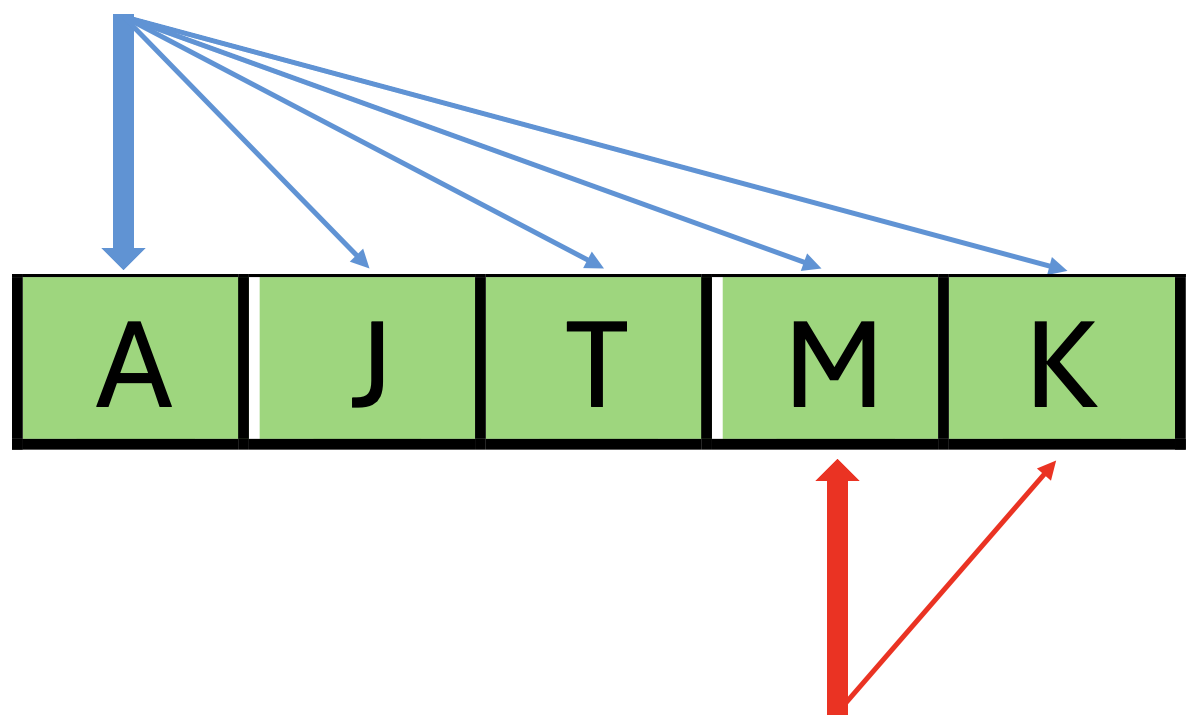
\includegraphics[width=0.5\textwidth]{005_ChercheDupliq_Optim.png}
			\end{figure}
			Le nombre d'opérations effectué par cette fonction au pire sera donc (en ne regardant que celles qui dépendent de n) la somme suivante: n + (n-1) + (...) + 2 + 1. Ca vous rappelle quelque chose...? $1 + 2 + ... + n = \frac{n(n + 1)}{2} = \frac{1}{2} \times n^2 + \frac{1}{2} \times n$. Or on a dit que pour l'estimation de la complexité on ignore les facteur multiplicateurs constants -- donc la complexité est la même que dans la version non-optimisée, quadratique: $\mathcal{O}(n^2)$.
			
			Ca peut paraitre étrange mais c'est en fait logique: la complexité n'est pas un calcul précis d'une durée de traitement, mais une estimation de la quantité dont dépend l'évolution du temps de traitement -- et on comprend bien qu'une dépendance à $n^2$ ou à $\frac{1}{2} \times n^2$ revient au même: si n double, le temps de traitement quadruplera dans les deux cas.
		\end{alphenum}
		
	\end{MaReponse}

	\subsection{Et dans la vraie vie...?}
	On vient de voir les complexités constantes, linéaires, et quadratiques --- il en existe en fait de nombreuses autres, mais qui ne sont pas au programme de 1\textsuperscript{ère}. Leur importance vaut le coup d'être mentionnée -- et elle est évidente si l'on regarde ce graphique de croissance des principales fonctions utilisées dans les calculs de complexité.
	
	\begin{figure}[ht]
		\centering
		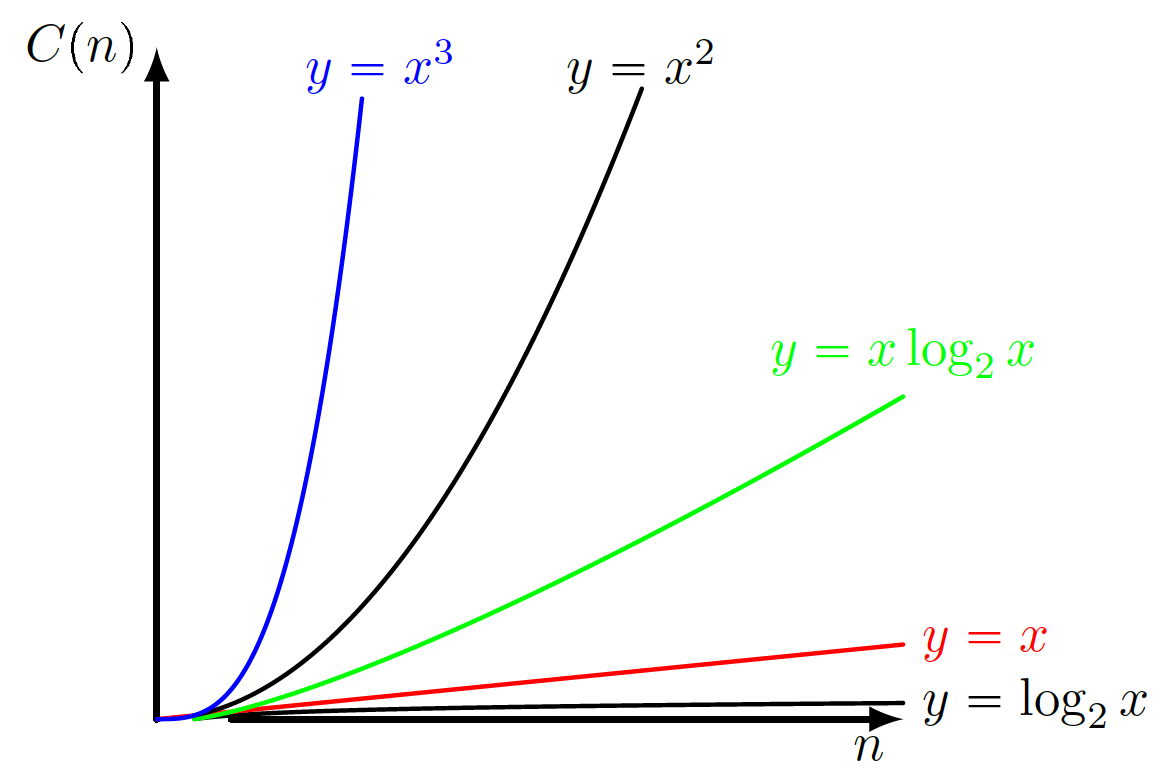
\includegraphics[width=0.8\textwidth]{002_Complexite.png}
	\end{figure}
	
	Le lien entre la complexité et les performances temporelles d'un algorithme devraient sembler évidents à la lecture de ce graphique, mais pour s'en convaincre davantage encore, il suffit de considérer ces tables (\textit{source: cours NSI Charles Poulmaire}). L'unité utilisée ("FLOPS") signifie "Floating-point operations per second" ou opération sur nombre flottant par seconde -- c'est donc bien une unité de mesure de la performance d'un ordinateur qui se rapporte directement à la complexité qui, elle, est un mesurée comme une estimation des opérations élémentaires.
	
	\begin{figure}[H]
		\centering
		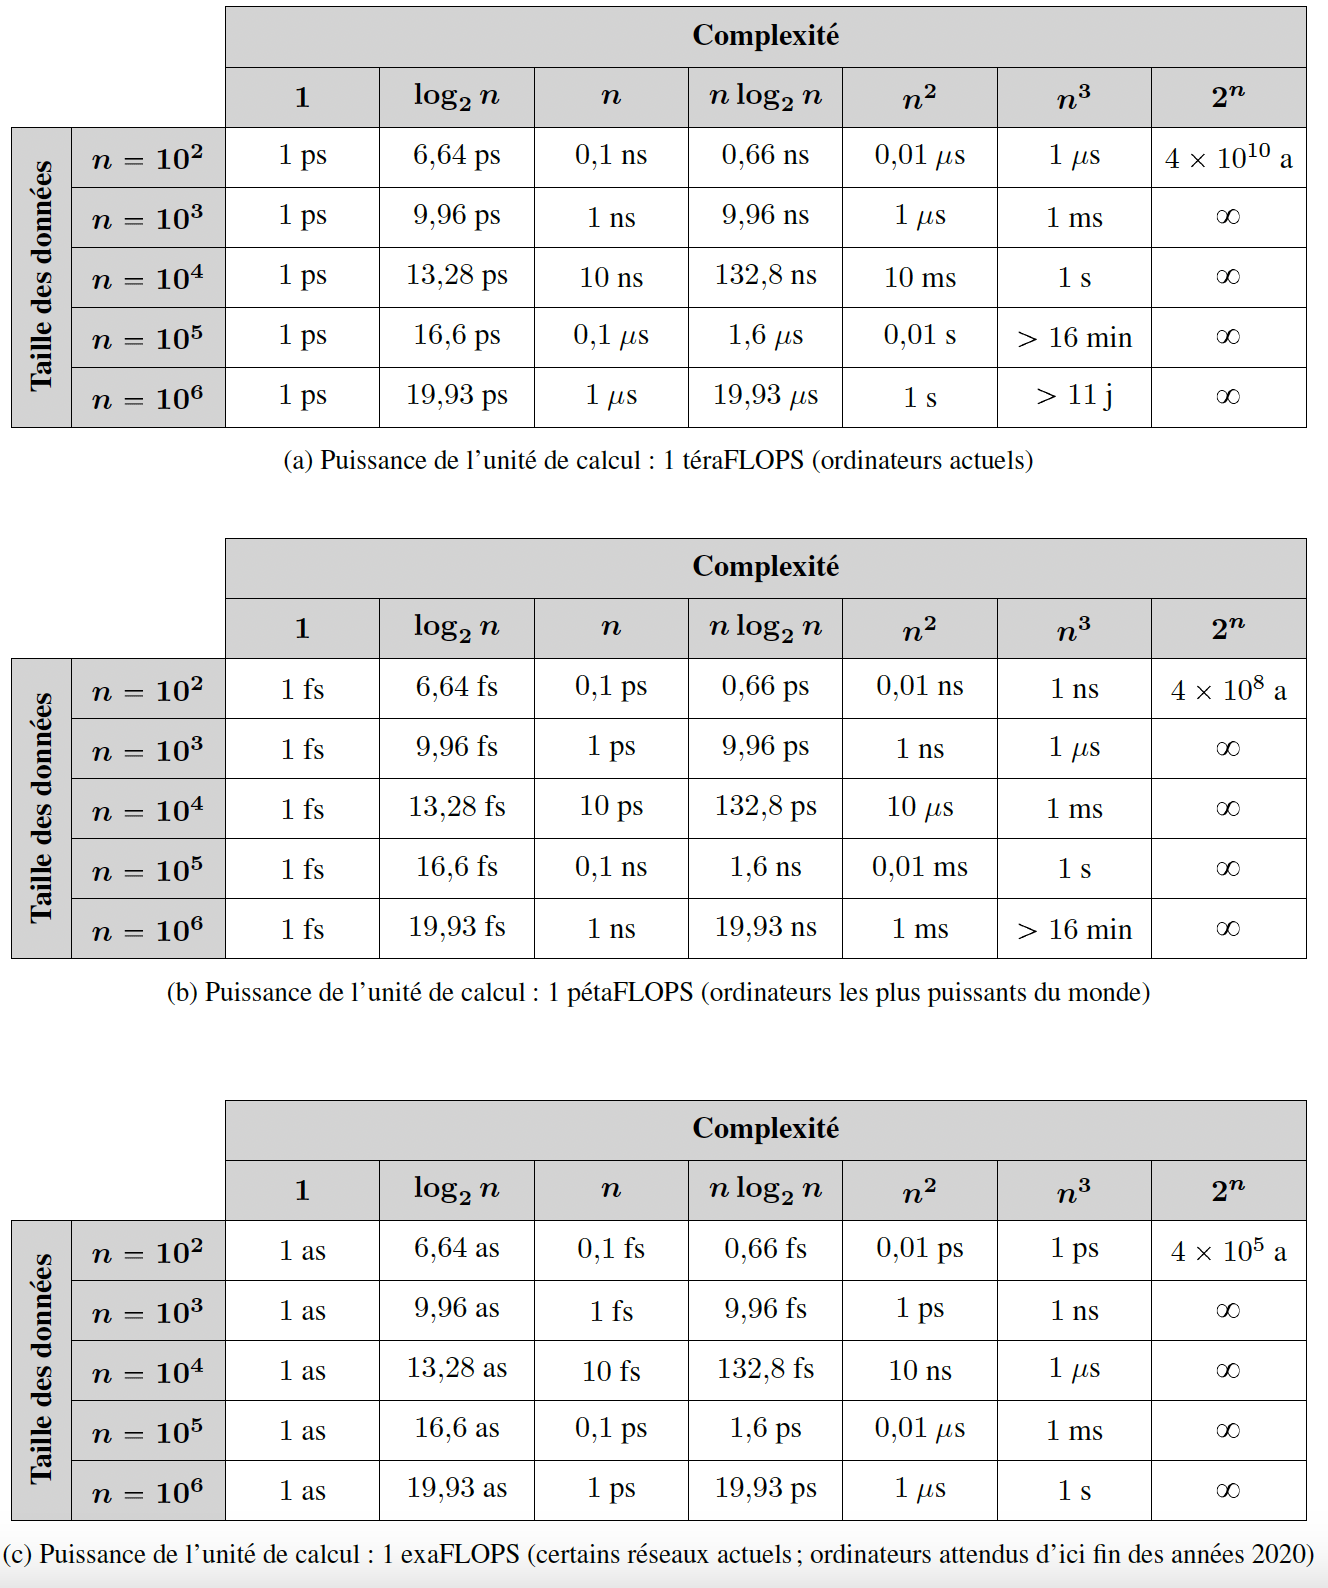
\includegraphics[width=\textwidth]{003_Performance.png}
	\end{figure}
	
	Les unités de temps utilisées ici  -- qui permettent également de mieux se rendre compte de la vitesse à laquelle évoluent les ordinateurs -- sont:
	\begin{description}
		\item[$\infty$] Infini -- temps que par convention on considère comme infini car irréalisable dans la réalité.
		\item[a] Année
		\item[j] Jour
		\item[min] Minute
		\item[s] Seconde
		\item [ms] Milliseconde -- $10^{-3}$ secondes -- un millième de seconde
		\item[$\mu$s] Microseconde -- $10^{-6}$ secondes -- un millième de seconde
		\item[ns] Nanoseconde -- $10^{-9}$ secondes -- un milliardième de seconde
		\item[ps] Picoseconde -- $10^{-12}$ secondes -- un mille milliardième de seconde
		\item[fs] Femtoseconde -- $10^{-15}$ secondes -- un million de milliardième de seconde
		\item[as] Attoseconde -- $10^{-18}$ secondes -- un milliard de milliardième de seconde
	\end{description}
	
	Et puisque l'on parle d'unités, je précise également les unités listées dans les libellés de ces trois tableaux qui décrivent la puissance de calcul des ordinateurs considérés:
	\begin{description}
		\item[téraFLOPS] $10^{12}$ opérations par seconde, soit mille milliards.
		\item[pétaFLOPS] $10^{15}$ opérations par seconde, soit un million de milliards (mille fois plus puissant que le premier).
		\item[exaFLOPS] $10^{18}$ opérations par seconde, soit un milliard milliards (mille fois plus puissant que le précédent, un million de fois plus que le premier).
	\end{description}
	
	\subsection{Complexité - à retenir}
	\begin{MonRet}
		Nous reviendrons dans les sections qui suivent sur les notions développées ici en les appliquant à certains algorithmes connus, mais ce qu'il faut retenir \textit{a minima} est:
		\begin{itemize}
			\item Notions de complexité spatiale et temporelle;
			\item Compréhension de l'importance du type dépendance entre le volume de données en entrée et le nombre d'opérations élémentaires à effectuer;
			\item Comptage des opérations élémentaires et estimation de la complexité -- être capable de résoudre des exercices comme ceux qui précèdent;
			\item En particulier être capable d'appliquer ces notions aux complexités constante ($\mathcal{O}(1)$), linéaire ($\mathcal{O}(n)$), et quadratique (\texttt{$\mathcal{O}(n^2)$}).
		\end{itemize}
	\end{MonRet}

	\pagebreak
	\section{Algorithmes de tri}
	\subsection{Pourquoi trier?}
	Imaginez que vous êtes dans une bibliothèque qui contient tous les livres qui étaient disponibles en France en 2019 -- ça fait quand même 810.130 livres différents\footnote{Source: \href{https://www.culture.gouv.fr/content/download/268286/3121285?v=1}{Document "Chiffres-clés du secteur du livre 2018-2019"}, Ministère de la Culture.}.
	\begin{wrapfigure}{l}{0.4\textwidth}
		\vspace{10pt} % Juste pour aligner un peu mieux l'image avec le paragraphe parce que je suis maniaque.
		
\includegraphics[scale=0.2]{006_Biblio.jpg}
	\end{wrapfigure}
	
	Ca ne paraît peut-être pas énorme, mais si on imagine qu'ils sont tous des livres de poche plus ou moins standard d'avec une tranche d'une épaisseur d'environ 1,9 cm, si on les range bout à bout sur une étagère, l'étagère devra mesurer plus de 15 kilomètres de long.... Alors si après ça je vous demande d'aller me chercher le livre \uline{Le Petit Prince} par Antoine de Saint-Exupéry, vous allez être \textit{très} mécontents si je précise que les livres sont rangés dans le désordre, et regretter qu'ils ne soient pas rangés par auteur puis par titre, par exemple.... 
	
	En informatique, c'est la même chose -- et on en a déjà un petit peu parlé dans le chapitre précédent, sur le traitement des données en table: si j'ai un tableau qui contient des milliers ou des millions d'informations (par exemple une liste de tous les clients d'Amazon, ou de tous les articles jamais publiés dans le journal Le Monde), il pourra être très lent d'en retrouver un si ils ne sont pas triés, mais à l'inverse ça pourra être relativement rapide s'ils le sont.
	
	Le problème se pose donc de \textit{comment} trier de grandes quantités de données -- et nous allons voir qu'il y a plusieurs solutions différentes. En 1\textsuperscript{ère}, nous allons aborder 3 algorithmes de tri différents:
	\begin{alphenum}
		\item Le tri par permutation;
		\item Le tri par sélection;
		\item Le tri par insertion.
	\end{alphenum}
	
	\subsection{Le tri par permutation ou "tri à bulles"}
	Considérez l'algorithme suivant:
	\begin{algorithmic}[1]
		\Require{$liste$ d'éléments ordonnables -- des nombres par exemple}
		\Ensure{?????}
		\Function{Tri1}{liste}
		\State N $\leftarrow$ longueur(liste)
		\For{$i$ allant de 1 à N-1}
		\If{$liste[i] > liste[i+1]$}
		\State Échanger Liste[i] et liste[i+1]
		\EndIf
		\EndFor
		\State\Return{$liste$}
		\EndFunction
	\end{algorithmic}
	
	\MaQuest{Que ferait cet algorithme sur la liste [2, 5, 3, 1]?}
	\begin{MaReponse}
		On a dans ce cas N = 4 et on peut décrire les états successifs de i et de liste en parcourant la boucle:
		\begin{center}
			\begin{tabular}{|c|c|c|c|}
				\hline
				\textbf{i}&\textbf{liste[j]}&\textbf{liste[j+1]}&\textbf{liste}\\
				\hline
				0 (avant la boucle)&N/A&N/A&[2, 5, 3, 1]\\
				\hline
				1&2&5&[2, 5, 3, 1]\\
				\hline
				2&5&3&[2, 3, 5, 1]\\
				\hline
				3&5&1&[2, 3, 1, 5]\\
				\hline
			\end{tabular}
		\end{center}
	\end{MaReponse}
		
	\MaQuest{Du coup que fait l'algorithme ci-dessus? Par quoi faudrait-il remplacer "?????" pour décrire ce qu'il renvoie?}
	\begin{MaReponse}
		On voit que cet algorithme, par permutations successives, fait systématiquement "remonter" l'élément le plus grand de la liste jusqu'à la dernière position du tableau. On pourrait donc décrire la sortie comme étant "liste, avec son plus grand élément placé en dernière position".
	\end{MaReponse}
	
	\MaQuest{Est-ce que cela donne des idées pour enrichir cet algorithme pour qu'il fasse un tri complet de la liste qu'il prend en entrée?}
	\begin{MaReponse}
		On constate qu'une exécution de cet algorithme permet de ramener le plus grand élément de la liste, où qu'il se trouve, en dernière position. Il n'est pas compliqué de se convaincre qu'en exécutant cet algorithme une fois encore sur le même tableau permettrait de ramener l'élément le deuxième plus grand de la liste en avant dernière position --- et par extension, N exécutions de l'algorithme permettrait d'aboutir à un tableau complètement trié!
		
		Si on applique ce principe au tableau précédent, on aurait, à l'issue de chaque exécution successive de l'algorithme:
		\begin{enumerate}
			\item \texttt{[2, 5, 3, 1]}
			\item \texttt{[2, 3, 1, 5]}
			\item \texttt{[2, 1, 3, 5]}
			\item \texttt{[1, 2, 3, 5]}
		\end{enumerate}
	\end{MaReponse}
	
	Appliquons cette conclusion à notre algorithme, traduisons-le en Python et considérons le résultat:
	\MonPython{007_TriBulles.py}
	
	\begin{MonAmp}{Explication video}
		\href{https://www.youtube.com/shorts/y2AghjB4Wxs?feature=share}{Youtube short} présentant le tri par sélection. Les variables de cette vidéo et celles du code ci-dessus sont les mêmes:
		\begin{itemize}
			\item \texttt{i} \quad \faExchange \quad \texttt{i}
			\item \texttt{j} \quad \faExchange \quad \texttt{j}
		\end{itemize}
	\end{MonAmp}
	
	\MaQuest{Quel est la complexité de cet algorithme?}
	
	\begin{MaReponse}
		La réponse en l'occurrence est assez immédiate: on a deux boucles imbriquées, chacune s'exécutant un nombre de fois directement dépendant de n --- donc on a affaire à une complexité en $\mathcal{O}(n^2)$, autrement dit quadratique.
	\end{MaReponse}
	
	\MaQuest{Allez -- une dernière question avant de conclure le chapitre: pourquoi à votre avis appelle-t-on ce tri par permutations "tri à bulles"?}
	
	\begin{MaReponse}
		\begin{tabular}{p{0.3\textwidth}p{0.6\textwidth}}
			\begin{minipage}{\linewidth}
				\begin{figure}[H]
					\centering
					
\includegraphics[width=0.5\textwidth]{007_Champagne.jpg}
				\end{figure}
			\end{minipage}
			&
			\begin{minipage}{\linewidth}
				C'est tout simplement l'image des bulles dans une boisson gazeuse comme du champagne qui, l'une après l'autre, remontent à la surface, à l'instar des valeurs les plus grandes de la liste qui "remontent" vers la fin.
			\end{minipage}
		\end{tabular}			
	\end{MaReponse}
		
	\subsection{Le tri par sélection}
	\subsubsection*{Présentation générale}
	Le tri par sélection s'inspire de la manière dont on trie des copies par ordre alphabétique des élèves:
	\begin{itemize}
		\item Au début, on tient toutes les copies dans la main gauche;
		\item On choisit la copie dont le nom est le premier dans l'ordre alphabétique, et on la place face retournée sur la table devant soi;
		\item On choisit ensuite parmi les copies restantes celle qui a le nom qui est le premier dans l'ordre alphabétique et on la place face retournée sur la précédente;
		\item On réitère ce procédé jusqu'à ce qu'on n'ait plus de copies dans la main gauche.
	\end{itemize}
	
	On se convainc donc facilement du fait que les copies présentes sur la table à tout instant sont triées.
	
	Le tri par sélection fonctionne de manière similaire au détail près qu'il n'utilise pas deux "lieux" (la main et la table) -- que l'on ne fait qu'échanger les éléments à l'intérieur de la table. A chaque étape du tri, on a:
	\begin{itemize}
		\item Le tableau est séparé en deux parties une partie triée "à gauche" (indices les plus petits) et une partie non triée "à droite".
		\begin{figure}[H]
			\centering
			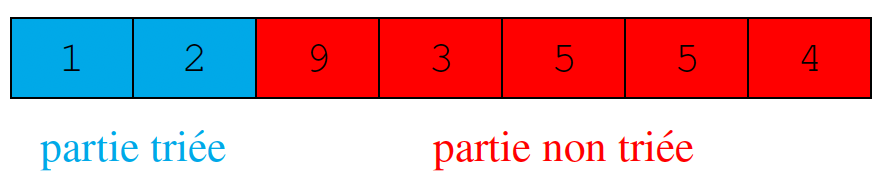
\includegraphics[width=0.45\textwidth]{008_TriSel1.png}
		\end{figure}
		\item On choisit le plus petit élément de la partie non triée et on le place au début de la partie non triée de telle sorte que la partie triée soit augmentée d'un élément et la partie non triée soit diminuée d'un élément.
		\begin{figure}[H]
			\centering
			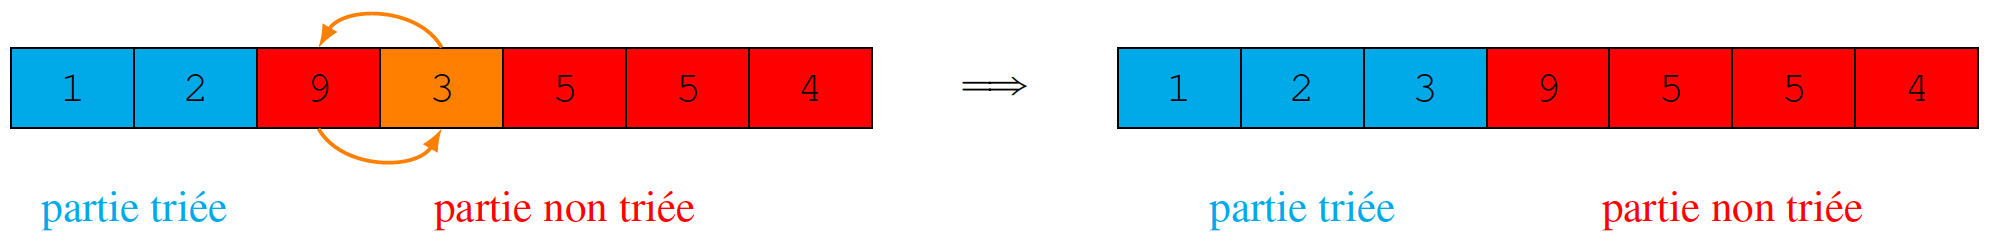
\includegraphics[width=0.9\textwidth]{009_TriSel2.png}
		\end{figure}
		\item On poursuit ainsi jusqu'à avoir parcouru toute la table.
	\end{itemize}
	
	Voyons l'application de cet algorithme de bout en bout à un exemple concret, la liste \texttt{[9,5,1,3,5,2,4]}:
	
	\begin{center}
		\begin{tabular}{c c}
			\multicolumn{2}{c}{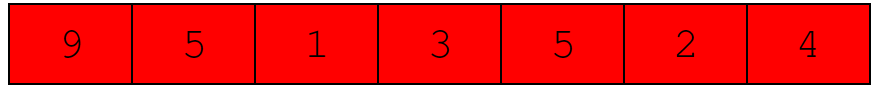
\includegraphics[width=0.5\textwidth]{010_TriSelEx1.png}} \\
			\multicolumn{2}{c}{\parbox{0.5\textwidth}{\centering A: table dans son état initial}} \\
			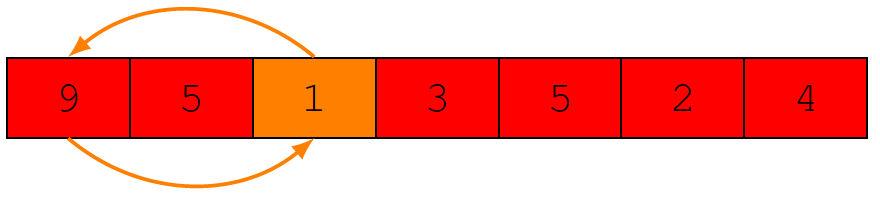
\includegraphics[width=0.5\textwidth]{011_TriSelEx2.png} & 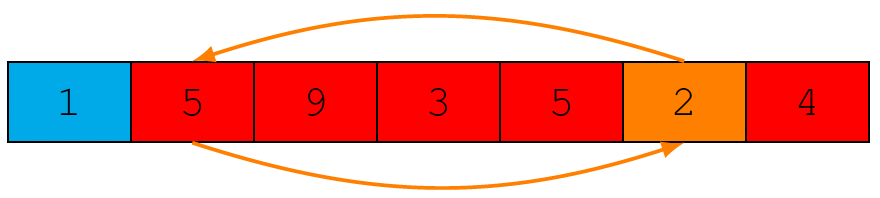
\includegraphics[width=0.5\textwidth]{012_TriSelEx3.png} \\
			\begin{minipage}{0.5\textwidth}
				B: On déplace le minimum (1) en première position. 
			\end{minipage} & 
			\begin{minipage}{0.5\textwidth}
				C: On déplace le minimum suivant (2) en deuxième position.
			\end{minipage} \\
			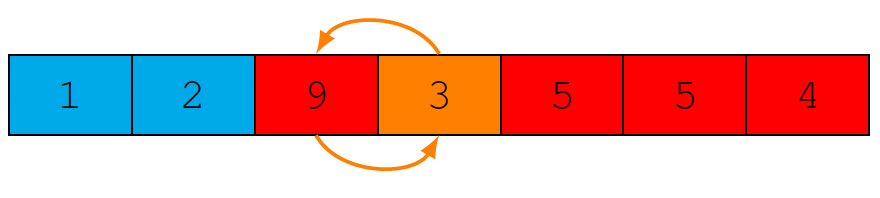
\includegraphics[width=0.5\textwidth]{013_TriSelEx4.png} & 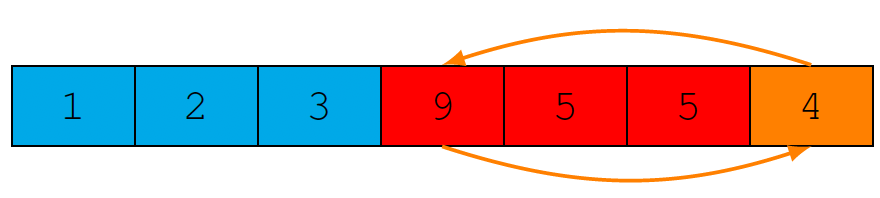
\includegraphics[width=0.5\textwidth]{014_TriSelEx5.png} \\
			\begin{minipage}{0.5\textwidth}
				D: On déplace le minimum suivant (3) en troisième position.
			\end{minipage} & 
			\begin{minipage}{0.5\textwidth}
				E: On déplace le minimum suivant (4) en quatrième position.
			\end{minipage} \\
			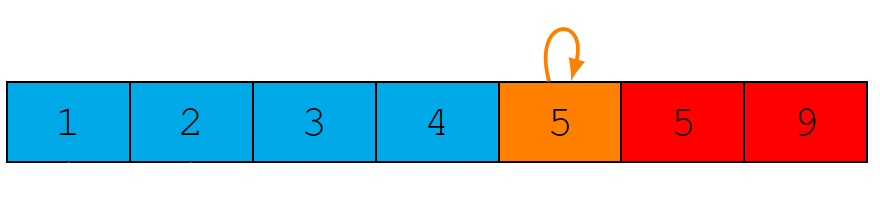
\includegraphics[width=0.5\textwidth]{015_TriSelEx6.png} & 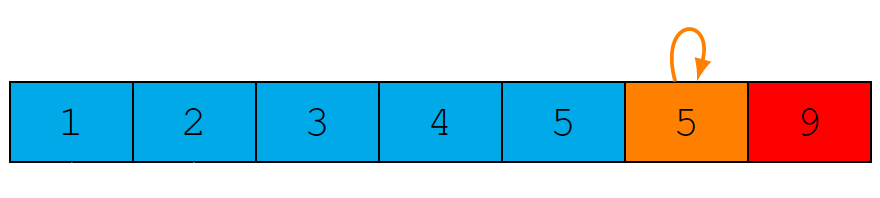
\includegraphics[width=0.5\textwidth]{016_TriSelEx7.png} \\
			\begin{minipage}{0.5\textwidth}
				F: On échange le minimum suivant (5) avec lui-même puisqu'il est déjà en place.
			\end{minipage} & 
			\begin{minipage}{0.5\textwidth}
				G: On échange le minimum suivant (5) avec lui-même puisqu'il est déjà en place.
			\end{minipage} \\
			\multicolumn{2}{c}{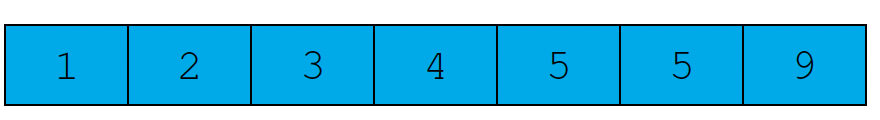
\includegraphics[width=0.5\textwidth]{017_TriSelEx8.png}} \\
			\multicolumn{2}{c}{\parbox{0.5\textwidth}{\centering H: table dans son état final}} \\
		\end{tabular}
	\end{center}
	
	\subsubsection*{Algorithme}
	\MaQuest{Sur la base de la description ci-dessus comment s'écrit cet algorithme en pseudo-code?}
	\begin{MaReponse}
		Exprimé en pseudo-code cet algorithme s'écrit ainsi:
		
		\begin{algorithmic}[1]
			\Require{$tab$, une liste}
			\Ensure{$tab$, triée}
			\Function{TriSelection}{tab}
			\State n $\leftarrow$ longueur(tab)
			\For{$p$ allant de 1 à (n-1)}
			\State pmin $\leftarrow$ p
			\For{$j$ allant de (p+1) à n}
			\If{$tab[j] < tab[pmin]$}
			\Comment{On a trouvé un nouveau min}
			\State $pmin$ $\leftarrow j$
			\EndIf
			\EndFor
			\State Échanger tab[pmin] et tab[p]
			\EndFor
			\State\Return{$tab$}
			\EndFunction
		\end{algorithmic}
		
		Le compteur p correspond à l'indice du premier élément de la partie non triée (position à laquelle il faut déplacer le plus petit élément de la partie non triée) et la variable pmin correspond à l’indice du plus petit élément de la partie non triée. On a ainsi le schéma suivant:
		\begin{figure}[H]
			\centering
			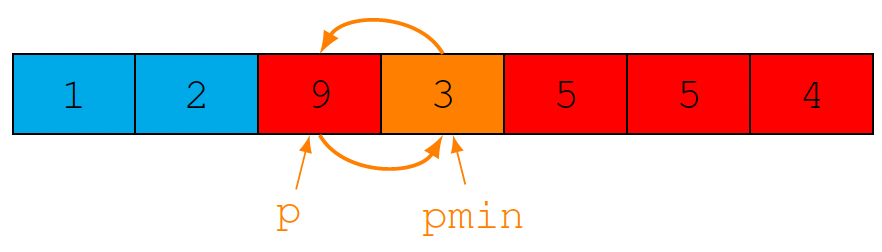
\includegraphics[width=0.45\textwidth]{018_TriSel3.png}
		\end{figure}
	\end{MaReponse}
	
	\begin{MonAmp}{Explication video}
		\href{https://www.youtube.com/shorts/HRwi5gwlB0U?feature=share}{Youtube short} présentant le tri par sélection. Les correspondances entre les variables de cette vidéo et celles du pseudo-code ci-dessus sont:
		\begin{itemize}
			\item \texttt{i} \quad \faExchange \quad \texttt{p}
			\item \texttt{j} \quad \faExchange \quad \texttt{j}
			\item \texttt{min} \quad \faExchange \quad \texttt{pmin}
		\end{itemize}
	\end{MonAmp}
	
	\subsubsection*{Preuve \& Complexité}
	\textbf{\uline{Terminaison}}: l'algorithme est composé de boucles pour dont la fin dépend, dans les deux cas, de \texttt{n}, longueur du tableau en entrée, qui ne varie pas: on connaît donc le nombre de répétitions, et donc l'algorithme se termine.
	
	\textbf{\uline{Correction partielle}}: l'algorithme préserve l'invariant de boucle suivant: "si $p \geq 1$, \texttt{tab} est trié entre les indices 1 et $p - 1$ , et tous les éléments restants sont supérieurs ou égaux à \texttt{tab[p-1]}".
	
	\textbf{\uline{Complexité}}: Dans la boucle interne (\texttt{pour j allant de (p+1) à n}), on effectue $n - p$ comparaisons. $p$ variant de 1 à (n-1) on en effectue donc successivement: $n-1$ (pour $p = 1$), puis $n-2$ (pour $p = 2$), puis (...), puis 2 (pour $p = n-2$), et enfin une seule (pour $p = n-1$). La complexité de l'algorithme s'exprime donc:
	\[
	1 + 2 + \text{(...)} + (n-2) + (n-1) = \frac{n(n-1)}{2} = \frac{1}{2}n^2 - \frac{1}{2}n
	\]
	On peut donc en conclure que la complexité de cet algorithme est quadratique, en $\mathcal{O}(n^2)$.
	
	\begin{MonExo}{Codage du tri par sélection}
		Vous fondant sur le pseudo-code ci-dessus, coder une fonction \texttt{TriSel(tab)} qui effectue le tri par sélection d'une liste passée en argument.
	\end{MonExo}
	\begin{MaReponse}
		\MonPython{008_TrSel.py}
	\end{MaReponse}
	
	\subsection{Tri par insertion}
	\subsubsection*{Présentation générale}
	Le tri par insertion s'inspire de la manière dont la plupart des gens trient les cartes à jouer qu'ils ont en main (pour rendre l'explication lisible on va imaginer ici que toutes les cartes sont de la même couleur -- il s'agit donc ici juste de les trier par ordre croissant):
	\begin{itemize}
		\item Au début, on tient toutes ses cartes dans le désordre;
		\item On regarde la deuxième en partant de la gauche: et si elle est de valeur supérieure ou égale à la première on la laisse en place; dans le cas contraire on la ramène en première position;
		\item On poursuit ainsi: on regarde à chaque fois la carte suivante, on la laisse en place si elle est supérieure à celle qui est juste à sa gauche, on la place au bon endroit dans la partie gauche de la main dans le cas contraire;
		\item On réitère ce procédé jusqu'à avoir placé la carte la plus à droite.
	\end{itemize}
	
	On se convainc donc facilement du fait que les cartes présentes à gauche de la main à tout instant sont triées.
	
	Le tri par insertion fonctionne de manière similaire. A chaque étape du tri, on a:
	\begin{itemize}
		\item Le tableau est séparé en deux parties: une partie triée que l'on suppose à gauche et une partie non triée que l’on suppose à droite;
		\begin{figure}[H]
			\centering
			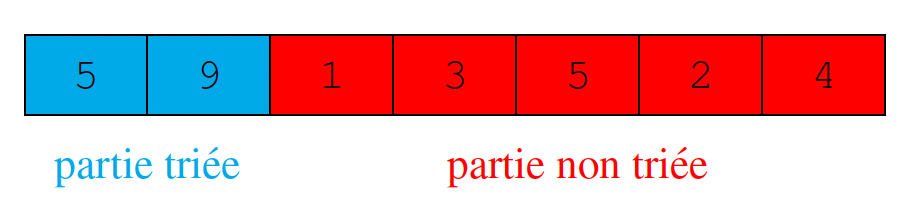
\includegraphics[width=0.45\textwidth]{019_TriIns1.png}
		\end{figure}
		\item On insère le premier élément de la partie non triée à sa place dans la partie triée en décalant vers la droite tous les éléments de la partie triée qui lui sont supérieurs afin que la partie triée soit augmentée d'un élément et la partie non triée soit diminuée d’un élément.
		\begin{figure}[H]
			\centering
			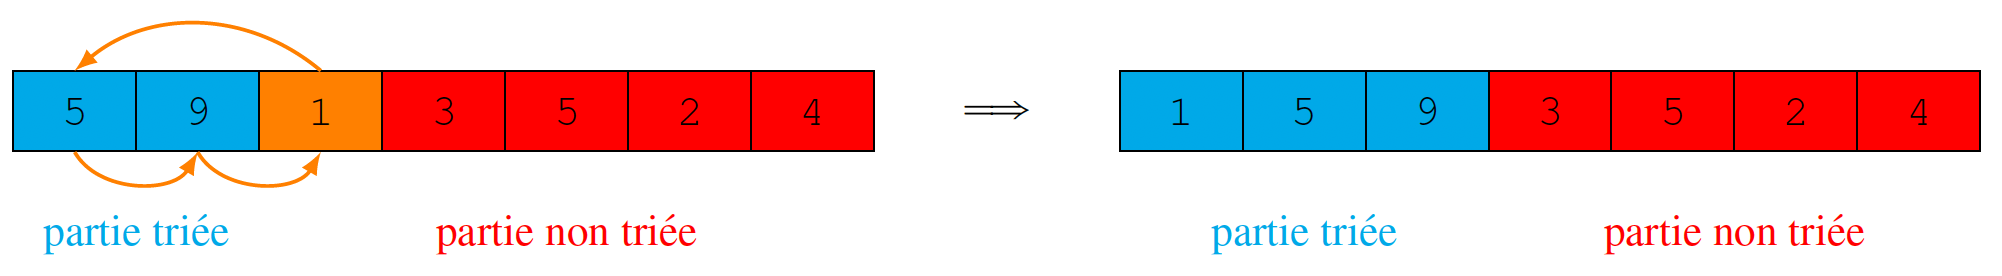
\includegraphics[width=0.9\textwidth]{020_TriIns2.png}
		\end{figure}
		\item On poursuit ainsi jusqu'à avoir parcouru toute la table.
	\end{itemize}
	
	Voyons l'application de cet algorithme de bout en bout à un exemple concret, la même liste que celle que l'on a utilisée pour le tri par sélection,  \texttt{[9,5,1,3,5,2,4]}:
	
	\begin{center}
		\begin{tabular}{c c}
			\multicolumn{2}{c}{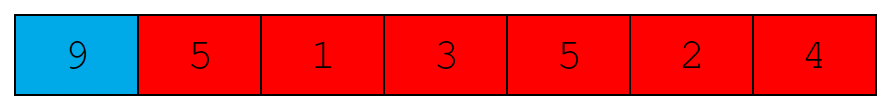
\includegraphics[width=0.5\textwidth]{021_TriSelIns1.png}} \\
			\multicolumn{2}{c}{\parbox{0.5\textwidth}{\centering A: table dans son état initial}} \\
			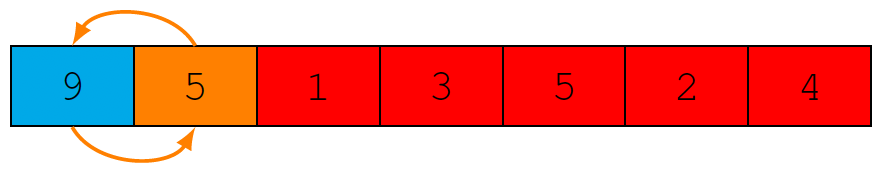
\includegraphics[width=0.5\textwidth]{022_TriSelIns2.png} & 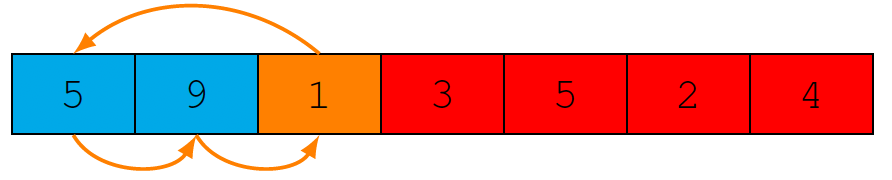
\includegraphics[width=0.5\textwidth]{023_TriSelIns3.png} \\
			\begin{minipage}{0.5\textwidth}
				B: On regarde le deuxième élément (5), on "l'insère" à sa place -- en l'occurrence au début de la liste; on effectue donc un échange.
			\end{minipage} & 
			\begin{minipage}{0.5\textwidth}
				C: On insère l'élément suivant (1), toujours en début de liste -- il faut donc décaler les deux éléments déjà triés "vers la droite" (donc augmenter la valeur de leurs indices).
			\end{minipage} \\
			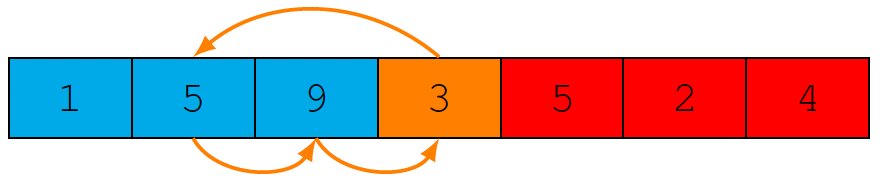
\includegraphics[width=0.5\textwidth]{024_TriSelIns4.png} & 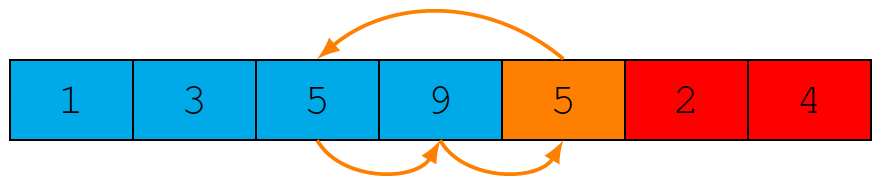
\includegraphics[width=0.5\textwidth]{025_TriSelIns5.png} \\
			\begin{minipage}{0.5\textwidth}
				D: On insère l'élément suivant (3) en deuxième position -- et on décale les éléments triés qui suivent.
			\end{minipage} & 
			\begin{minipage}{0.5\textwidth}
				E: Même chose avec le 5...
			\end{minipage} \\
			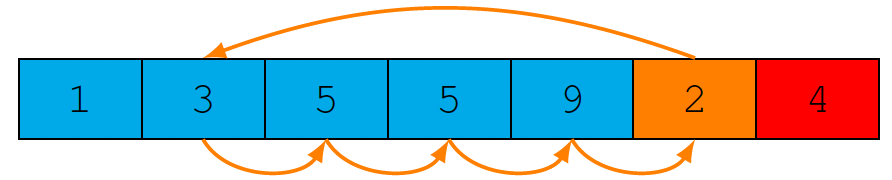
\includegraphics[width=0.5\textwidth]{026_TriSelIns6.png} & 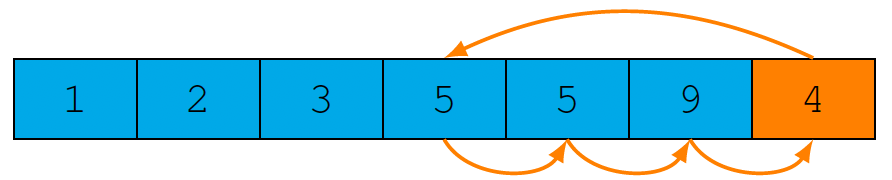
\includegraphics[width=0.5\textwidth]{027_TriSelIns7.png} \\
			\begin{minipage}{0.5\textwidth}
				F: On insère à présent le 2, et ce sont quatre éléments qu'il faut décaler vers la droite.
			\end{minipage} & 
			\begin{minipage}{0.5\textwidth}
				G: On termine avec le 4.
			\end{minipage} \\
			\multicolumn{2}{c}{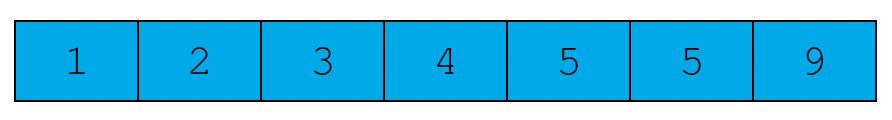
\includegraphics[width=0.5\textwidth]{028_TriSelIns8.png}} \\
			\multicolumn{2}{c}{\parbox{0.5\textwidth}{\centering H: table dans son état final}} \\
		\end{tabular}
	\end{center}
	
	\subsubsection*{Algorithme}
	\MaQuest{Sur la base de la description ci-dessus comment s'écrit cet algorithme en pseudo-code? (Attention! Pour ne pas "perdre" de valeur, vous allez devoir utiliser une variable temporaire pendant que vous faites le décalage d'indices qui précède l'insertion)}
	\begin{MaReponse}
		Exprimé en pseudo-code cet algorithme s'écrit ainsi:
		
		\begin{algorithmic}[1]
			\Require{$tab$, une liste}
			\Ensure{$tab$, triée}
			\Function{TriInsertion}{tab}
			\State n $\leftarrow$ longueur(tab)
			\For{$i$ allant de 2 à n}
			\State temp $\leftarrow$ tab[i]
			\State p $\leftarrow$ i
			\While{$p > 1$ et tab[p-1] > temp}
			
			\Comment{On remonte le tableau jusqu'à trouver la place de tab[i]}
			\State tab[p] $\leftarrow$ tab[p-1]
			\State p $\leftarrow$ p-1
			\EndWhile
			\State tab[p] $\leftarrow$ temp
			\Comment{On a trouvé la place de tab[i]}
			\EndFor
			\State\Return{$tab$}
			\EndFunction
		\end{algorithmic}
		
		Le compteur i correspond à l'indice du premier élément de la partie non triée et la variable p correspond à l'indice de la position où il faut insérer \texttt{tab[i]} dans la partie triée. On a ainsi le schéma suivant:
		\begin{figure}[H]
			\centering
			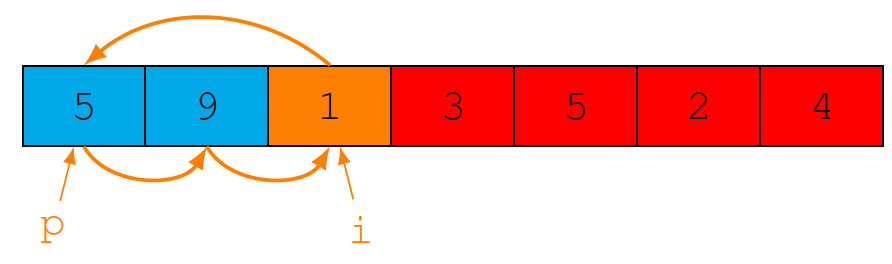
\includegraphics[width=0.45\textwidth]{029_TriIns3.png}
		\end{figure}
	\end{MaReponse}
	
	\begin{MonAmp}{Explication video}
		\href{https://www.youtube.com/shorts/ZZ-Oz1IFfPg?feature=share}{Youtube short} présentant le tri par insertion. La vidéo utilise des indices décalés par rapport à ce qui est présenté ici donc ne vous attardez pas trop sur les variables en tant que telles (vous risqueriez de vous y perdre), mais regardez le procédé dépeint dans la vidéo qui, lui, est le bon. Pour être complet cependant, les correspondances entre les variables de cette vidéo et celles du pseudo-code ci-dessus sont:
		\begin{itemize}
			\item \texttt{key} \quad \faExchange \quad \texttt{temp} (ou \texttt{tab[i]})
			\item \texttt{j} \quad \faExchange \quad \texttt{p-1}
		\end{itemize}
	\end{MonAmp}
	
	\subsubsection*{Preuve \& Complexité}
	\textbf{\uline{Terminaison}}: 
	\begin{itemize}
		\item La boucle \texttt{pour} sera de toute manière réalisée $(n-1)$ fois, et $n$ ne varie pas -- donc elle se terminera.
		\item La boucle \texttt{tant que} doit être vérifiée au moyen d'un variant de boucle -- $p$ en l'occurrence: $p$ est initialisé à $i$ --- donc est strictement positif --- et décroît strictement. Donc la boucle se termine également.
	\end{itemize}
	
	\textbf{\uline{Correction partielle}}: l'algorithme préserve l'invariant de boucle suivant: "si $i \geq 2$, \texttt{tab} est trié entre les indices 1 et $i - 1$ , et tous les éléments restants restent à trier".
	
	\textbf{\uline{Complexité}}: Dans le pire des cas (si la liste est triée au départ par ordre décroissant), la boucle interne (\texttt{tant que}) effectue $2i$ comparaisons (donc 4, puis 6, puis (...), puis $(2n - 2)$, puis enfin 2n). La complexité de l'algorithme s'exprime donc:
	\begin{align*}
	4 + 6 + \text{(...)} + (2n-2) + 2n &= 2 \times (2 + 3 + \text{(...)} + (n-1) + n) \\
	&= 2 \times \frac{(n-1)\times (n+2)}{2} \\
	&= n^2 + n - 2
	\end{align*}
	On peut donc en conclure que la complexité de cet algorithme est quadratique, en $\mathcal{O}(n^2)$.
	
	\begin{MonExo}{Codage du tri par sélection}
		Vous fondant sur le pseudo-code ci-dessus, coder une fonction \texttt{TriIns(tab)} qui effectue le tri par insertion d'une liste passée en argument.
	\end{MonExo}
	\begin{MaReponse}
		\MonPython{009_TriIns.py}
	\end{MaReponse}
	
	\subsection{Comparaisons entre ces algorithmes...}
	\subsubsection*{Complexité "au mieux"}
	On a dit plus haut dans ce cours que les calculs de complexité se font dans des configurations "au pire" -- donc dans les cas où, à taille de données en entrée équivalente, les données sont telles que l'algorithme effectuera un maximum d'opérations. Mais si, comme ils semble que ce soit le cas ici, on a des algorithmes apparemment équivalents, est-ce qu'on ne pourrait pas regarder ce qu'il se passe "au mieux" pour les départager?
	
	Considérons de nouveau le tri par insertion et imaginons que les données en entrée sont déjà triées. En ce cas, on voit bien que la condition \texttt{tab[p-1] > temp} n'est \textit{jamais} satisfaite, et que donc seule la boucle externe, la boucle \texttt{pour} influence la complexité. Or celle-ci est effectuée $(n-1)$ fois, donc on se retrouvera avec une complexité linéaire, en $\mathcal{O}(n)$.
	
	Cette considération a-t-elle un intérêt? Imaginez que vous mettiez bout à bout deux listes, toutes deux déjà triées, une (appelée "t") très longue, et une (appelée "s") très courte, comme dans le schéma ci-dessous:
	\begin{figure}[H]
		\centering
		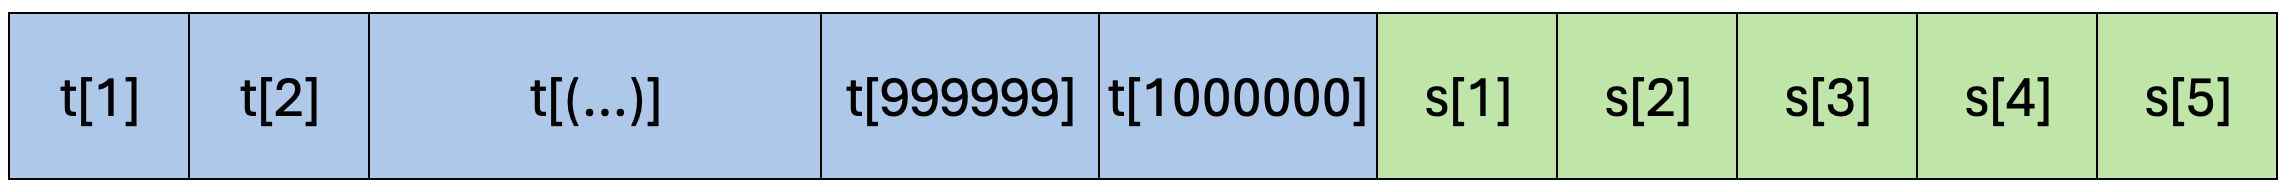
\includegraphics[width=0.9\textwidth]{030_AuMieux.png}
	\end{figure}
	On se convainc aisément que dans ce cas la vaste majorité des itérations se fera sans passage dans la boucle internet et que seules les quelques dernières donneront lieu à un réel tri, ce qui réduira considérablement le temps de traitement par rapport à un tri par sélection où toutes les comparaisons seront effectuées quoi qu'il arrive.
	
	\textit{Deux remarques au sujet de ce qui précède:
	\begin{enumerate}
		\item Vous noterez que dans cet exemple le fait de mettre la liste courte \textbf{après} la liste longue est fondamental -- c'est typiquement le genre de question d'optimisation qu'il faut régulièrement se poser;
		\item En pratique cette situation ne se poserait pas en ces termes -- je vous la présente ici simplement pour illustrer une différence de performances entre ces deux algorithmes de tri.
	\end{enumerate}}
	
	\subsubsection*{Stabilité d'un tri}
	Un autre critère de comparaison entre différents algorithmes de tri est leur stabilité -- on entend par là dans quel ordre se retrouveront les éléments égaux entre eux une fois la table triée. Il y a deux possibilités:
	\begin{itemize}
		\item Tri stable: les éléments conservent quoiqu'il arrive le même ordre qu'ils avaient dans la table initiale;
		\item Tri instable: les éléments peuvent changer d'ordre par rapport à la table initiale.
	\end{itemize}
	L'importance de ce critère peut se comprendre lorsque l'on considère des tris suivant plusieurs axes. Imaginons qu'on a une liste d'albums de musique qui est déjà triée par noms d'album et qu'on veut ensuite lui appliquer un tri par nom d'artiste: un tri stable fera que les albums d'un même artiste resteront en ordre alphabétique, tandis qu'un tri instable ne le garantira pas.
	
	Imaginons à présent qu'on considère une liste de bouteilles triée par marque, représentée ainsi:
	\begin{figure}[H]
		\centering
		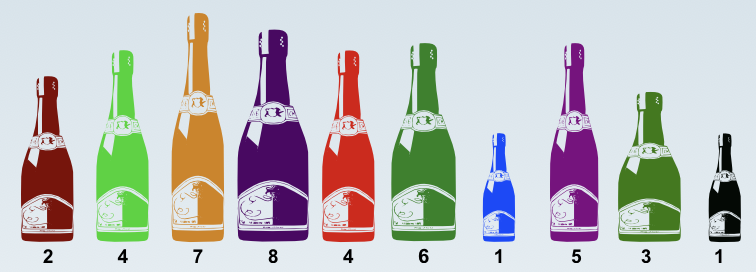
\includegraphics[width=0.5\textwidth]{031_BtlInit.png}
	\end{figure}
	
	On souhaite la trier par contenance de bouteilles. Un tri instable donnera par exemple:
	\begin{figure}[H]
		\centering
		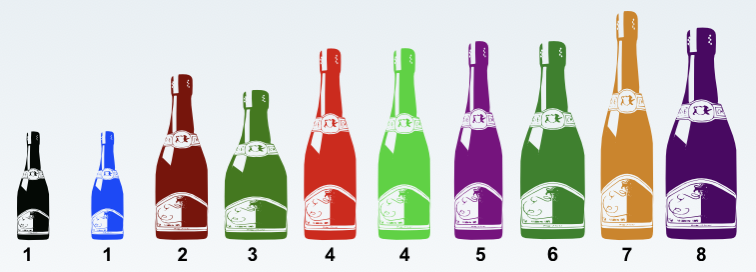
\includegraphics[width=0.5\textwidth]{032_BtlInstable.png}
	\end{figure}
	
	Tandis qu'un tri stable donnera (unique solution possible):
	\begin{figure}[H]
		\centering
		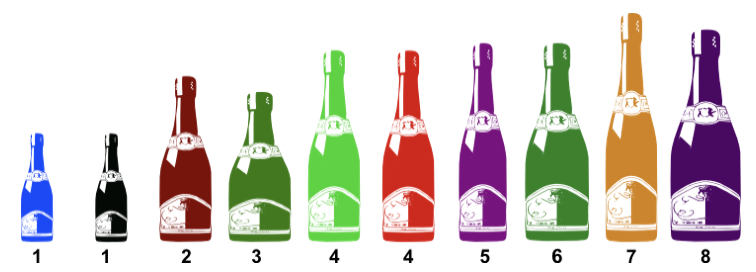
\includegraphics[width=0.5\textwidth]{033_BtlStable.png}
	\end{figure}
	
	\textit{(observez les bouteilles de contenance 1 et 4 dans cet exemple)}

	\subsubsection*{Avantages et inconvénients}
	
	\begin{small}	
		\begin{tabular}{|c|p{4cm}|p{4cm}|p{4cm}|}
			\hline
			&Tri à bulles&Tri par sélection&Tri par insertion\\
			\hline
			Avantages&
			\begin{minipage}[t]{\linewidth}
				\begin{zeromgitem}
					\item Simple à comprendre
					\item Facile à implémenter
				\end{zeromgitem}
			\end{minipage} &
			\begin{minipage}[t]{\linewidth}
				\begin{zeromgitem}
					\item Performant sur de petites listes
					\item Espace mémoire constant
				\end{zeromgitem}
			\end{minipage} &
			\begin{minipage}[t]{\linewidth}
				\begin{zeromgitem}
					\item Stable
					\item Bonne performance sur des listes déjà partiellement triées
				\end{zeromgitem}
			\end{minipage} \\
			\hline
		\end{tabular}
	\end{small}
	
	\subsection{Tris fournis par Python}
	Bon, soyons honnêtes... Les tris que l'on a étudiés ici ont pour but principal de vous initier à l'étude de l'algorithmique -- en pratique ils ne sont pas très performants et il en existe d'autres de bien mieux (notamment certains que l'on étudiera en Terminale pour ceux d'entre vous qui conserveront la spécialité NSI).
	
	Parmi les fonctions de tri beaucoup plus performantes il en est deux qui vous sont directement fournies par Python: la fonction \texttt{sorted()} qui fournit une copie triée de votre tableau; et la méthode \texttt{t.sort()} qui elle effectue une tri \textit{en place} d'un tableau \texttt{t} (c'est-à-dire qu'elle modifie le tableau lui même pour le trier). Ces deux fonctions effectuent un tri stable.
	
	Illustration de leur fonctionnement:
	\begin{figure}[H]
		\centering
		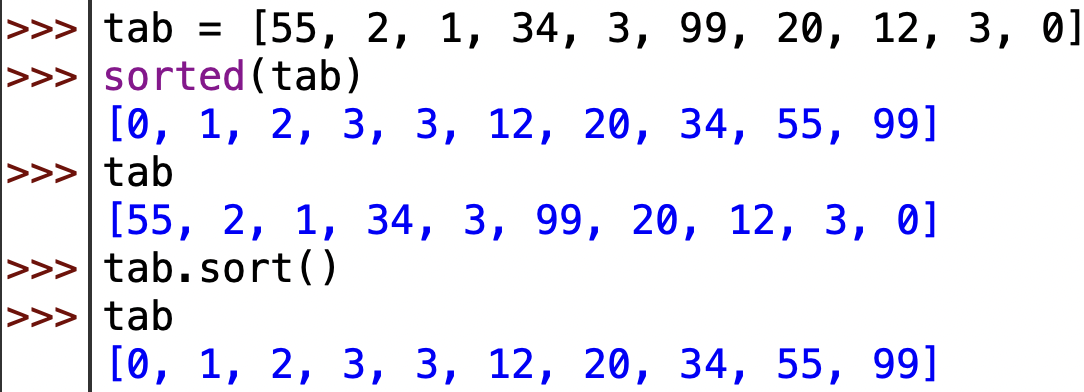
\includegraphics[width=0.7\textwidth]{034_SortSorted.png}
	\end{figure}
	
	\subsection{Algorithmes de tri -- à retenir}
		\begin{MonRet}
		De ces algorithmes de tri il faut que vous reteniez:
		\begin{itemize}
			\item Les principes de base -- vous devez être capables de les expliquer si on vous en donne le pseudo-code ou le code;
			\item La complexisté et le calcul de son ordre de grandeur ($\mathcal{O}()$);
			\item Le fonctionnement -- tel qu'on l'a décrit ici, qui doit vous permettre de résoudre des exercices comme ceux qui sont inclus dans le cahier d'exercices d'entraînement;
			\item Sommairement, les avantages et inconvénients de chacun d'entre eux.
		\end{itemize}
	\end{MonRet}
	
\end{document}


%Eléments manquants:
